% Options for packages loaded elsewhere
% Options for packages loaded elsewhere
\PassOptionsToPackage{unicode}{hyperref}
\PassOptionsToPackage{hyphens}{url}
\PassOptionsToPackage{dvipsnames,svgnames,x11names}{xcolor}
%
\documentclass[
  12pt,
  letterpaper,
  DIV=11,
  numbers=noendperiod]{scrreprt}
\usepackage{xcolor}
\usepackage[margin=1in]{geometry}
\usepackage{amsmath,amssymb}
\setcounter{secnumdepth}{5}
\usepackage{iftex}
\ifPDFTeX
  \usepackage[T1]{fontenc}
  \usepackage[utf8]{inputenc}
  \usepackage{textcomp} % provide euro and other symbols
\else % if luatex or xetex
  \usepackage{unicode-math} % this also loads fontspec
  \defaultfontfeatures{Scale=MatchLowercase}
  \defaultfontfeatures[\rmfamily]{Ligatures=TeX,Scale=1}
\fi
\usepackage{lmodern}
\ifPDFTeX\else
  % xetex/luatex font selection
\fi
% Use upquote if available, for straight quotes in verbatim environments
\IfFileExists{upquote.sty}{\usepackage{upquote}}{}
\IfFileExists{microtype.sty}{% use microtype if available
  \usepackage[]{microtype}
  \UseMicrotypeSet[protrusion]{basicmath} % disable protrusion for tt fonts
}{}
\usepackage{setspace}
\makeatletter
\@ifundefined{KOMAClassName}{% if non-KOMA class
  \IfFileExists{parskip.sty}{%
    \usepackage{parskip}
  }{% else
    \setlength{\parindent}{0pt}
    \setlength{\parskip}{6pt plus 2pt minus 1pt}}
}{% if KOMA class
  \KOMAoptions{parskip=half}}
\makeatother
% Make \paragraph and \subparagraph free-standing
\makeatletter
\ifx\paragraph\undefined\else
  \let\oldparagraph\paragraph
  \renewcommand{\paragraph}{
    \@ifstar
      \xxxParagraphStar
      \xxxParagraphNoStar
  }
  \newcommand{\xxxParagraphStar}[1]{\oldparagraph*{#1}\mbox{}}
  \newcommand{\xxxParagraphNoStar}[1]{\oldparagraph{#1}\mbox{}}
\fi
\ifx\subparagraph\undefined\else
  \let\oldsubparagraph\subparagraph
  \renewcommand{\subparagraph}{
    \@ifstar
      \xxxSubParagraphStar
      \xxxSubParagraphNoStar
  }
  \newcommand{\xxxSubParagraphStar}[1]{\oldsubparagraph*{#1}\mbox{}}
  \newcommand{\xxxSubParagraphNoStar}[1]{\oldsubparagraph{#1}\mbox{}}
\fi
\makeatother


\usepackage{longtable,booktabs,array}
\usepackage{calc} % for calculating minipage widths
% Correct order of tables after \paragraph or \subparagraph
\usepackage{etoolbox}
\makeatletter
\patchcmd\longtable{\par}{\if@noskipsec\mbox{}\fi\par}{}{}
\makeatother
% Allow footnotes in longtable head/foot
\IfFileExists{footnotehyper.sty}{\usepackage{footnotehyper}}{\usepackage{footnote}}
\makesavenoteenv{longtable}
\usepackage{graphicx}
\makeatletter
\newsavebox\pandoc@box
\newcommand*\pandocbounded[1]{% scales image to fit in text height/width
  \sbox\pandoc@box{#1}%
  \Gscale@div\@tempa{\textheight}{\dimexpr\ht\pandoc@box+\dp\pandoc@box\relax}%
  \Gscale@div\@tempb{\linewidth}{\wd\pandoc@box}%
  \ifdim\@tempb\p@<\@tempa\p@\let\@tempa\@tempb\fi% select the smaller of both
  \ifdim\@tempa\p@<\p@\scalebox{\@tempa}{\usebox\pandoc@box}%
  \else\usebox{\pandoc@box}%
  \fi%
}
% Set default figure placement to htbp
\def\fps@figure{htbp}
\makeatother


% definitions for citeproc citations
\NewDocumentCommand\citeproctext{}{}
\NewDocumentCommand\citeproc{mm}{%
  \begingroup\def\citeproctext{#2}\cite{#1}\endgroup}
\makeatletter
 % allow citations to break across lines
 \let\@cite@ofmt\@firstofone
 % avoid brackets around text for \cite:
 \def\@biblabel#1{}
 \def\@cite#1#2{{#1\if@tempswa , #2\fi}}
\makeatother
\newlength{\cslhangindent}
\setlength{\cslhangindent}{1.5em}
\newlength{\csllabelwidth}
\setlength{\csllabelwidth}{3em}
\newenvironment{CSLReferences}[2] % #1 hanging-indent, #2 entry-spacing
 {\begin{list}{}{%
  \setlength{\itemindent}{0pt}
  \setlength{\leftmargin}{0pt}
  \setlength{\parsep}{0pt}
  % turn on hanging indent if param 1 is 1
  \ifodd #1
   \setlength{\leftmargin}{\cslhangindent}
   \setlength{\itemindent}{-1\cslhangindent}
  \fi
  % set entry spacing
  \setlength{\itemsep}{#2\baselineskip}}}
 {\end{list}}
\usepackage{calc}
\newcommand{\CSLBlock}[1]{\hfill\break\parbox[t]{\linewidth}{\strut\ignorespaces#1\strut}}
\newcommand{\CSLLeftMargin}[1]{\parbox[t]{\csllabelwidth}{\strut#1\strut}}
\newcommand{\CSLRightInline}[1]{\parbox[t]{\linewidth - \csllabelwidth}{\strut#1\strut}}
\newcommand{\CSLIndent}[1]{\hspace{\cslhangindent}#1}



\setlength{\emergencystretch}{3em} % prevent overfull lines

\providecommand{\tightlist}{%
  \setlength{\itemsep}{0pt}\setlength{\parskip}{0pt}}



 


\usepackage{xcolor}
\usepackage{amsthm,amsmath,amsfonts,amssymb,float,caption,subcaption}
\usepackage{booktabs,longtable,array}
\KOMAoption{captions}{tableheading}
\makeatletter
\@ifpackageloaded{bookmark}{}{\usepackage{bookmark}}
\makeatother
\makeatletter
\@ifpackageloaded{caption}{}{\usepackage{caption}}
\AtBeginDocument{%
\ifdefined\contentsname
  \renewcommand*\contentsname{Table of contents}
\else
  \newcommand\contentsname{Table of contents}
\fi
\ifdefined\listfigurename
  \renewcommand*\listfigurename{List of Figures}
\else
  \newcommand\listfigurename{List of Figures}
\fi
\ifdefined\listtablename
  \renewcommand*\listtablename{List of Tables}
\else
  \newcommand\listtablename{List of Tables}
\fi
\ifdefined\figurename
  \renewcommand*\figurename{Figure}
\else
  \newcommand\figurename{Figure}
\fi
\ifdefined\tablename
  \renewcommand*\tablename{Table}
\else
  \newcommand\tablename{Table}
\fi
}
\@ifpackageloaded{float}{}{\usepackage{float}}
\floatstyle{ruled}
\@ifundefined{c@chapter}{\newfloat{codelisting}{h}{lop}}{\newfloat{codelisting}{h}{lop}[chapter]}
\floatname{codelisting}{Listing}
\newcommand*\listoflistings{\listof{codelisting}{List of Listings}}
\makeatother
\makeatletter
\makeatother
\makeatletter
\@ifpackageloaded{caption}{}{\usepackage{caption}}
\@ifpackageloaded{subcaption}{}{\usepackage{subcaption}}
\makeatother
\usepackage{bookmark}
\IfFileExists{xurl.sty}{\usepackage{xurl}}{} % add URL line breaks if available
\urlstyle{same}
\hypersetup{
  pdftitle={Appendix: Quantifying Hidden Exploitation},
  pdfauthor={{[}Author(s) anonymised for review{]}},
  colorlinks=true,
  linkcolor={blue},
  filecolor={Maroon},
  citecolor={BrickRed},
  urlcolor={blue},
  pdfcreator={LaTeX via pandoc}}


\title{Appendix: Quantifying Hidden Exploitation}
\usepackage{etoolbox}
\makeatletter
\providecommand{\subtitle}[1]{% add subtitle to \maketitle
  \apptocmd{\@title}{\par {\large #1 \par}}{}{}
}
\makeatother
\subtitle{Online Supplementary Materials for Social Indicators Research
Submission}
\author{{[}Author(s) anonymised for review{]}}
\date{11 July 2026}
\begin{document}
\maketitle

\renewcommand*\contentsname{Table of contents}
{
\hypersetup{linkcolor=}
\setcounter{tocdepth}{2}
\tableofcontents
}

\setstretch{1.15}
\bookmarksetup{startatroot}

\chapter*{Preface}\label{preface}
\addcontentsline{toc}{chapter}{Preface}

\markboth{Preface}{Preface}

This appendix accompanies the main paper. Appendix A documents the
codebook and how the composite risk index and the five binary
exploitation indicators are constructed. Appendix B lists the
survey-instrument questions used to elicit ego- and alter-based reports
for each indicator. Appendix C describes the three-step bootstrap
procedure used for the NSUM confidence intervals. Appendix D reports the
sensitivity and robustness analyses summarised in the main paper.

All data and replication code are available at
\href{\%5BOSF\%20view-only\%20URL\%20redacted\%20for\%20anonymised\%20review;\%20will\%20be\%20provided\%20upon\%20request\%5D}{OSF}.
The composite risk index and all indicator variables are constructed in
\texttt{R/data\_processing/02-data\_preparation.R} via
\texttt{create\_comparable\_indicators()}.

\cleardoublepage
\phantomsection
\addcontentsline{toc}{part}{Appendices}
\appendix

\chapter{Variable Codebook and Indicator Definitions}\label{sec-a}

This section documents the composite risk index construction, the five
binary exploitation indicators used as the primary prevalence outcomes,
and the key RDS variables.

\section{Composite Risk Index}\label{sec-a-composite}

The composite risk index aggregates all eleven ILO indicators of forced
labour into a single continuous measure (range 0--0.99). The index is a
formative additive composite: an individual is exposed to exploitation
if any of the indicators is present, and the indicators are constitutive
rather than reflective of an underlying severity construct. Polarity is
uniform across categories. Each of the eleven ILO indicator categories
contributes equally to the composite (maximum 0.09 per category, so the
total maximum possible score is 11 × 0.09 = 0.99). Within a category,
the 0.09 is distributed evenly across the sub-questions used to code
that category (0.09 for one sub-question, 0.045 each for two, 0.03 each
for three, 0.0225 each for four). All eleven ILO indicators contribute
equally to the composite. The medium/strong severity labels (following
International Labour Organization (\citeproc{ref-hard24-ilo}{2024})) are
used for reporting; they do not enter the composite's arithmetic.

Two further evidentiary markers --- payment below the national living
wage (Category 12) and NRM-referral history (Category 13) --- are
reported as separate binary flags and are \textbf{not} included in the
composite, because their direct evidentiary status under UK policy makes
them more useful when read independently.

Table~\ref{tbl-composite} lists each of the eleven ILO categories that
enter the composite alongside the survey items used to code them, the
coding rules, and the maximum weight per category. Categories 12 and 13
are shown at the bottom of the table for completeness but do not enter
the composite score.

\begin{longtable}[]{@{}
  >{\raggedright\arraybackslash}p{(\linewidth - 8\tabcolsep) * \real{0.2000}}
  >{\raggedright\arraybackslash}p{(\linewidth - 8\tabcolsep) * \real{0.2000}}
  >{\raggedright\arraybackslash}p{(\linewidth - 8\tabcolsep) * \real{0.2000}}
  >{\raggedright\arraybackslash}p{(\linewidth - 8\tabcolsep) * \real{0.2000}}
  >{\raggedright\arraybackslash}p{(\linewidth - 8\tabcolsep) * \real{0.2000}}@{}}
\caption{Composite Risk Index: ILO indicator categories, survey items,
coding rules, and sub-weights. All eleven ILO indicator categories carry
the same maximum category weight of 0.09; this 0.09 is split evenly
across the sub-questions used to code the category (0.09 for one, 0.045
each for two, 0.03 each for three, 0.0225 each for four sub-questions).
The total maximum composite score is therefore 11 × 0.09 = 0.99. The
medium/strong severity labels in column 2 follow the ILO handbook on
forced-labour surveys (\citeproc{ref-hard24-ilo}{International Labour
Organization, 2024}); the shorter ILO operational-indicators
publications (\citeproc{ref-ILO11-indicators}{International Labour
Organization, 2012}, \citeproc{ref-int25-ilo}{2025}) list the eleven
indicators without publishing this severity ranking, and the labels do
not scale the composite weights. Categories 12 and 13 are reported as
separate binary flags and are excluded from the
composite.}\label{tbl-composite}\tabularnewline
\toprule\noalign{}
\begin{minipage}[b]{\linewidth}\raggedright
\#
\end{minipage} & \begin{minipage}[b]{\linewidth}\raggedright
ILO Indicator (severity)
\end{minipage} & \begin{minipage}[b]{\linewidth}\raggedright
Survey item(s)
\end{minipage} & \begin{minipage}[b]{\linewidth}\raggedright
Coding rule
\end{minipage} & \begin{minipage}[b]{\linewidth}\raggedright
Max weight
\end{minipage} \\
\midrule\noalign{}
\endfirsthead
\toprule\noalign{}
\begin{minipage}[b]{\linewidth}\raggedright
\#
\end{minipage} & \begin{minipage}[b]{\linewidth}\raggedright
ILO Indicator (severity)
\end{minipage} & \begin{minipage}[b]{\linewidth}\raggedright
Survey item(s)
\end{minipage} & \begin{minipage}[b]{\linewidth}\raggedright
Coding rule
\end{minipage} & \begin{minipage}[b]{\linewidth}\raggedright
Max weight
\end{minipage} \\
\midrule\noalign{}
\endhead
\bottomrule\noalign{}
\endlastfoot
1 & Abuse of vulnerability (medium) & Q29 (5a1): Forced to do work
against will; Q51 (5d2-a): Unpaid tasks & Q29: 0/1/2 → 0.045; Q51: 0 →
0.045 & 0.09 \\
2 & Deception (medium) & Q45 (5c2): Forced/deceived/threatened into poor
conditions & Q45: 0 → 0.09 & 0.09 \\
3 & Restriction of movement (medium) & Q32 (5a4): Could not leave
premises; Q46 (5c3): Stay overnight permanently & Q32: 0/1/2 → 0.045;
Q46: 2 or 3 → 0.045 & 0.09 \\
4 & Isolation (medium) & Q65: Have friends outside work & Q65: 1 (No) →
0.09 & 0.09 \\
5 & Physical and sexual violence (strong) & Q44 (5c1):
Abuse/harassment/physical violence; Q44 (5c1-b): Sexual violence & Q44
(5c1): 0 → 0.045; Q44 (5c1-b): 0 → 0.045 & 0.09 \\
6 & Intimidation and threats (strong) & Q47 (5c4): Employer
threatened/intimidated & Q47: 0/1/2 → 0.09 & 0.09 \\
7 & Retention of identity documents (strong) & Q70 (5f2):
Travel/identity docs withheld & Q70: 0/1/2 → 0.09 & 0.09 \\
8 & Withholding of wages (medium) & Q42 (5b7): Pay ever withheld & Q42:
0/1/2 → 0.09 & 0.09 \\
9 & Debt bondage (medium) & Q39 (5b4): Earnings to pay off debt to
helper & Q39: 0 → 0.09 & 0.09 \\
10 & Abusive working and living conditions (medium) & Q48 (5c5):
Verbally abused; Q63 (5d10): Lack of privacy; Q72 (5f4): Safe/healthy
environment; Q76 (5f8): Access to food/water/sanitation & Q48: 0/1/2 →
0.0225; Q63: 0/1/2 → 0.0225; Q72: 2 or 3 → 0.0225; Q76: 1/2/3 → 0.0225 &
0.09 \\
11 & Excessive overtime (medium) & Q16 (3b): Weekly hours; Q61 (5d8):
Weekly rest ≥ 24h; Q62 (5d9): Excessive overtime felt & Q16: 6 or 7 →
0.03; Q61: 2 or 3 → 0.03; Q62: 0/1/2 → 0.03 & 0.09 \\
12 & Payment below national living wage \emph{(separate binary)} & Q36
(5b1): Hourly pay before tax & Q36: 0/1/2 (below £10.42/hr) → 1 &
Reported separately \\
13 & NRM-referral indicator \emph{(separate binary)} & Q80 (5f12):
Advised to enter National Referral Mechanism & Q80: 0 or 1 → 1 &
Reported separately \\
\end{longtable}

\section{Five Binary Exploitation Indicators}\label{sec-a-binary}

The five binary indicators are the primary prevalence outcomes for both
the ego-based RDS and alter-based NSUM analyses. All are binary (0/1).
Multi-category RDS responses are recoded so that affirmative answers →
1, Never/no access → 0, and ``Don't know''/``Prefer not to say'' → NA.
Composite RDS indicators combine sub-questions using logical OR (any
affirmative response across sub-questions → 1). NSUM count variables
(number of domestic workers known with the characteristic) are converted
to binary (\textgreater{} 0 → 1). Table~\ref{tbl-binary} summarises the
mapping from each binary indicator to its ILO classification, the survey
items that code it, and the coding rule applied.

\begin{longtable}[]{@{}
  >{\raggedright\arraybackslash}p{(\linewidth - 6\tabcolsep) * \real{0.2500}}
  >{\raggedright\arraybackslash}p{(\linewidth - 6\tabcolsep) * \real{0.2500}}
  >{\raggedright\arraybackslash}p{(\linewidth - 6\tabcolsep) * \real{0.2500}}
  >{\raggedright\arraybackslash}p{(\linewidth - 6\tabcolsep) * \real{0.2500}}@{}}
\caption{Five Binary Exploitation Indicators: ILO classification, survey
questions, and coding rules.}\label{tbl-binary}\tabularnewline
\toprule\noalign{}
\begin{minipage}[b]{\linewidth}\raggedright
Binary indicator
\end{minipage} & \begin{minipage}[b]{\linewidth}\raggedright
ILO classification
\end{minipage} & \begin{minipage}[b]{\linewidth}\raggedright
Survey item(s)
\end{minipage} & \begin{minipage}[b]{\linewidth}\raggedright
Coding rule
\end{minipage} \\
\midrule\noalign{}
\endfirsthead
\toprule\noalign{}
\begin{minipage}[b]{\linewidth}\raggedright
Binary indicator
\end{minipage} & \begin{minipage}[b]{\linewidth}\raggedright
ILO classification
\end{minipage} & \begin{minipage}[b]{\linewidth}\raggedright
Survey item(s)
\end{minipage} & \begin{minipage}[b]{\linewidth}\raggedright
Coding rule
\end{minipage} \\
\midrule\noalign{}
\endhead
\bottomrule\noalign{}
\endlastfoot
Document withholding & Strong (Category 7) & Q70 (5f2): Travel/identity
docs withheld & Q70: 0/1/2 → 1 \\
Threats and abuse & Strong (Categories 5+6) & Q45 (5c2):
Forced/deceived/threatened; Q47 (5c4): Intimidated; Q48 (5c5): Verbally
abused & Any of: Q45=0; Q47=0/1/2; Q48=0/1/2 → 1 \\
Pay issues & Medium (Categories 8+9) & Q39 (5b4): Debt bondage; Q42
(5b7): Pay withheld & Either Q39=0 or Q42=0/1/2 → 1 \\
Excessive hours & Medium (Category 11) & Q61 (5d8): Weekly rest
\textless{} 24h; Q62 (5d9): Excessive overtime & Either Q61=2/3 or
Q62=0/1/2 → 1 \\
Limited access to help & Auxiliary & Q78 (5f10): Knows where to get help
(reverse-coded) & Q78 indicating no access → 1 \\
\end{longtable}

\section{Key RDS Variables}\label{sec-a-rds}

Table~\ref{tbl-rds-vars} lists the variables used by the RDS estimation
pipeline (\texttt{R/analysis/03-rds\_estimation.R} and downstream
scripts). The \texttt{id}/\texttt{recruiter.id} pair defines the
recruitment network on which all RDS weighting and successive-sampling
procedures operate; \texttt{q13} is the reported network-degree variable
used to weight respondents in inverse proportion to their reported
degree; \texttt{wave} and \texttt{nationality\_cluster} are stratifying
variables used in diagnostic plots and subgroup sensitivity analyses.
All variables are constructed in
\texttt{R/data\_processing/02-data\_preparation.R}.

\begin{longtable}[]{@{}
  >{\raggedright\arraybackslash}p{(\linewidth - 6\tabcolsep) * \real{0.2500}}
  >{\raggedright\arraybackslash}p{(\linewidth - 6\tabcolsep) * \real{0.2500}}
  >{\raggedright\arraybackslash}p{(\linewidth - 6\tabcolsep) * \real{0.2500}}
  >{\raggedright\arraybackslash}p{(\linewidth - 6\tabcolsep) * \real{0.2500}}@{}}
\caption{Key RDS Variables: variable name, type, definition, and survey
source.}\label{tbl-rds-vars}\tabularnewline
\toprule\noalign{}
\begin{minipage}[b]{\linewidth}\raggedright
Variable
\end{minipage} & \begin{minipage}[b]{\linewidth}\raggedright
Type
\end{minipage} & \begin{minipage}[b]{\linewidth}\raggedright
Definition
\end{minipage} & \begin{minipage}[b]{\linewidth}\raggedright
Source
\end{minipage} \\
\midrule\noalign{}
\endfirsthead
\toprule\noalign{}
\begin{minipage}[b]{\linewidth}\raggedright
Variable
\end{minipage} & \begin{minipage}[b]{\linewidth}\raggedright
Type
\end{minipage} & \begin{minipage}[b]{\linewidth}\raggedright
Definition
\end{minipage} & \begin{minipage}[b]{\linewidth}\raggedright
Source
\end{minipage} \\
\midrule\noalign{}
\endhead
\bottomrule\noalign{}
\endlastfoot
id & Numeric & Unique respondent identifier & --- \\
recruiter.id & Numeric & id of recruiter; −1 = seed & --- \\
referral\_1 through referral\_5 & Numeric & ids of up to five recruits &
--- \\
q13 (2f) & Numeric (count) & Personal network size: number of other
domestic workers known with contact details. Used as degree variable in
RDS weighting and NSUM denominator. & Q13 \\
1a\_eligibility & Binary & Worked as domestic worker in past 12 months &
Q1a \\
wave & Numeric (0, 1, 2, \ldots) & Recruitment wave; 0 = seed; k =
recruited by wave-(k−1) respondent & Derived \\
nationality\_cluster & Categorical (4 levels) & Filipino, Latinx,
British, Other & Q3, Q5 \\
\end{longtable}

\chapter{Survey Questions and Comparable Ego/Alter
Indicators}\label{sec-b}

This section documents the full wording and response options for the
ego-based (RDS) and alter-based (NSUM) survey questions underlying each
of the five binary exploitation indicators. Ego-based questions ask
respondents about their own experiences; alter-based questions ask what
respondents observe in the domestic workers they know personally. This
matched ego/alter pairing is the foundation of the dual-method design.
All question numbers refer to the original survey instrument (\emph{The
Nature and Extent of Labour Exploitation among Domestic Workers in the
UK}, administered via OnlineSurveys, {[}Institution anonymised for
review{]}).

Table~\ref{tbl-ego-alter-summary} gives a summary overview; the
subsections below provide the full question wording, response options,
and coding rules for each indicator pair.

\begin{longtable}[]{@{}
  >{\raggedright\arraybackslash}p{(\linewidth - 6\tabcolsep) * \real{0.2500}}
  >{\raggedright\arraybackslash}p{(\linewidth - 6\tabcolsep) * \real{0.2500}}
  >{\raggedright\arraybackslash}p{(\linewidth - 6\tabcolsep) * \real{0.2500}}
  >{\raggedright\arraybackslash}p{(\linewidth - 6\tabcolsep) * \real{0.2500}}@{}}
\caption{Comparable Ego/Alter Indicator Pairs --- Summary. Confidence
ratings reflect the closeness of the conceptual match between the ego
(RDS) and alter (NSUM) question
framings.}\label{tbl-ego-alter-summary}\tabularnewline
\toprule\noalign{}
\begin{minipage}[b]{\linewidth}\raggedright
Indicator
\end{minipage} & \begin{minipage}[b]{\linewidth}\raggedright
Ego (RDS) question(s)
\end{minipage} & \begin{minipage}[b]{\linewidth}\raggedright
Alter (NSUM) question
\end{minipage} & \begin{minipage}[b]{\linewidth}\raggedright
Confidence
\end{minipage} \\
\midrule\noalign{}
\endfirsthead
\toprule\noalign{}
\begin{minipage}[b]{\linewidth}\raggedright
Indicator
\end{minipage} & \begin{minipage}[b]{\linewidth}\raggedright
Ego (RDS) question(s)
\end{minipage} & \begin{minipage}[b]{\linewidth}\raggedright
Alter (NSUM) question
\end{minipage} & \begin{minipage}[b]{\linewidth}\raggedright
Confidence
\end{minipage} \\
\midrule\noalign{}
\endhead
\bottomrule\noalign{}
\endlastfoot
Document withholding & Q70 (5f2) & Q71 (5f3) & Highest \\
Pay/debt issues & Q39 (5b4) + Q42 (5b7) & Q43 (5b8) & High \\
Threats and abuse & Q45 (5c2) + Q47 (5c4) + Q48 (5c5) & Q49 (5c6) &
High \\
Excessive hours & Q61 (5d8) + Q62 (5d9) & Q64 (5d11) & Medium \\
Limited access to help & Q78 (5f10) reverse-coded & Q79 (5f11) &
Lower \\
\end{longtable}

\section{Document Withholding}\label{sec-b-doc}

\textbf{Ego-based --- Q70 (5f2):}

\begin{quote}
\emph{Has your employer, or their agent, withheld from you your travel
and identity documentation?}

Response options: Yes, always / Often / Sometimes / Never / I don't know
\end{quote}

\textbf{Alter-based --- Q71 (5f3):}

\begin{quote}
\emph{Do you know personally of any other domestic workers who do not
have access to their own travel and identity documents? If so, how many?
(Please indicate the number, or state `0' if this does not apply to
anyone you know.)}

Response: Integer count
\end{quote}

\textbf{Coding.} Ego: Q70 ∈ \{Yes always, Often, Sometimes\} → 1;
\{Never, I don't know\} → 0; missing → NA. Alter: Q71 \textgreater{} 0 →
1; Q71 = 0 → 0; missing → NA.

\textbf{Confidence: Highest.} The ego and alter questions are direct
mirror images of the same exploitation behaviour. The only difference is
perspective (self vs.~others), not concept or scope.

\section{Pay/Debt Issues}\label{sec-b-pay}

\textbf{Ego-based --- Q39 (5b4):}

\begin{quote}
\emph{Do you have to use some or all of what you earn to pay off a debt
to someone who helped you find work?}

Response options: Yes / No / I don't know
\end{quote}

\textbf{Ego-based --- Q42 (5b7):}

\begin{quote}
\emph{Has your pay ever been withheld by your employer?}

Response options: Yes, always / Often / Sometimes / Never / I don't know
\end{quote}

\textbf{Alter-based --- Q43 (5b8):}

\begin{quote}
\emph{Do you know personally of any other domestic workers who have
experienced problems with debt or pay? If so, how many? (Please indicate
the number, or state `0' if this does not apply to anyone you know.)}

Response: Integer count
\end{quote}

\textbf{Coding.} Ego: Q39 = Yes → 1; \{No, I don't know\} → 0 (debt
bondage component). Q42 ∈ \{Yes always, Often, Sometimes\} → 1; \{Never,
I don't know\} → 0 (pay withheld component). Composite
\texttt{pay\_issues\_rds}: logical OR --- Q39 = 1 OR Q42 = 1 → 1; both
NA → NA. Alter: Q43 \textgreater{} 0 → 1; Q43 = 0 → 0; missing → NA.

\textbf{Confidence: High.} The alter question (Q43) covers both debt and
pay problems, matching the combined ego indicator. Some conceptual
mismatch remains because the alter question aggregates two distinct ego
concepts into one.

\section{Threats and Abuse}\label{sec-b-threats}

\textbf{Ego-based --- Q45 (5c2):}

\begin{quote}
\emph{Have you been forced, deceived or threatened into poor working
conditions?}

Response options: Yes / No / Prefer not to say
\end{quote}

\textbf{Ego-based --- Q47 (5c4):}

\begin{quote}
\emph{Has your employer ever threatened or intimidated you?}

Response options: Yes / Often / Sometimes / Never / I don't know
\end{quote}

\textbf{Ego-based --- Q48 (5c5):}

\begin{quote}
\emph{Has your employer ever verbally abused you (e.g.~shouted,
insulted, tried to humiliate you, or called you names, etc.)?}

Response options: Yes, Often / Yes, Sometimes / Maybe once or twice /
Never / I don't know
\end{quote}

\textbf{Alter-based --- Q49 (5c6):}

\begin{quote}
\emph{Do you know personally of any other domestic workers that have had
any experiences related to the use of threat or force? If so, how many?
(Please indicate the number, or state `0' if this does not apply to
anyone you know.)}

Response: Integer count
\end{quote}

\textbf{Coding.} Ego: Q45 = Yes → 1; \{No, Prefer not to say\} → 0. Q47
∈ \{Yes, Often, Sometimes\} → 1; \{Never, I don't know\} → 0. Q48 ∈
\{Yes Often, Yes Sometimes, Maybe once or twice\} → 1; \{Never, I don't
know\} → 0. Composite \texttt{threats\_abuse\_rds}: logical OR --- any
of Q45/Q47/Q48 = 1 → 1; all three NA → NA. Alter: Q49 \textgreater{} 0 →
1; Q49 = 0 → 0; missing → NA.

\textbf{Confidence: High.} Q49 captures the combined concept of threat
and force, aligning with the three ego sub-questions. The ego composite
is slightly broader (it includes verbal abuse via Q48), so some scope
mismatch remains at the margin.

\section{Excessive Working Hours}\label{sec-b-hours}

\textbf{Ego-based --- Q61 (5d8):}

\begin{quote}
\emph{Does your weekly rest last longer than 24 hours consecutively?}

Response options: Yes, always / Often / Sometimes / Never / I don't know
\end{quote}

\textbf{Ego-based --- Q62 (5d9):}

\begin{quote}
\emph{How often have you worked overtime that you felt was excessive?}

Response options: Always / Often / Sometimes / Never / I don't know
\end{quote}

\textbf{Alter-based --- Q64 (5d11):}

\begin{quote}
\emph{Do you know personally of any other domestic workers who have
experienced any of the above related to labour rights? (Including
working excessive overtime, a failure to obtain daily or weekly breaks
or annual leave.) If so, how many? (Please indicate the number, or state
`0' if this does not apply to anyone you know.)}

Response: Integer count
\end{quote}

\textbf{Coding.} Ego: Q61 ∈ \{Sometimes, Never\} → 1 (indicates
\emph{inadequate} rest, i.e., rest rarely or never exceeds 24 h); \{Yes
always, Often, I don't know\} → 0. Q62 ∈ \{Always, Often, Sometimes\} →
1; \{Never, I don't know\} → 0. Composite
\texttt{excessive\_hours\_rds}: logical OR → 1 if either condition
present; both NA → NA. Alter: Q64 \textgreater{} 0 → 1; Q64 = 0 → 0;
missing → NA.

\textbf{Confidence: Medium.} Q64 explicitly includes \emph{annual leave}
(``a failure to obtain \ldots{} annual leave'') which is not captured by
Q61 or Q62 on the ego side. This scope mismatch is the largest of the
five indicator pairs and is acknowledged as a limitation of the
comparable-indicator strategy.

\section{Limited Access to Help}\label{sec-b-help}

\textbf{Ego-based --- Q78 (5f10):}

\begin{quote}
\emph{Do you know who might help you if you are not being properly paid
or properly treated?}

Response options: Yes / No
\end{quote}

\textbf{Alter-based --- Q79 (5f11):}

\begin{quote}
\emph{Do you know personally of any other domestic workers who do NOT
know where to go for help? If so, how many? (Please indicate the number,
or state `0' if this does not apply to anyone you know.)}

Response: Integer count
\end{quote}

\textbf{Coding.} Ego: Q78 is reverse-coded --- Q78 = No → 1 (respondent
lacks access to help); Q78 = Yes → 0; missing → NA. Alter: Q79
\textgreater{} 0 → 1; Q79 = 0 → 0; missing → NA.

\textbf{Confidence: Lower.} Q78 directly reports the respondent's own
knowledge of available support, while Q79 asks the respondent to assess
\emph{others'} knowledge. The reverse-coding of Q78 aligns the polarity
(both = 1 signals vulnerability), but the alter question requires the
respondent to perceive and report on peers' states of knowledge --- a
different and more demanding cognitive task than self-report. The
conceptual match is therefore less direct than for the other four
indicators.

\section{General Data-Processing Notes}\label{sec-b-notes}

All five indicators are binary (0/1) after recoding. RDS multi-category
responses are recoded so that affirmative responses → 1, and
negative/unknown responses → 0 or NA as specified above. Composite RDS
indicators (pay/debt issues, threats and abuse, excessive hours) apply
logical OR: any single affirmative sub-response → indicator = 1; only if
\emph{all} sub-questions are missing does the composite take the value
NA. NSUM count variables are converted to binary: count \textgreater{} 0
→ 1; count = 0 → 0. These constructions are implemented in
\texttt{create\_comparable\_indicators()} in
\texttt{R/data\_processing/02-data\_preparation.R}, following the
comparable-indicator specification agreed between the authors in
November 2024.

\chapter{Three-Step Bootstrap Procedure}\label{sec-c}

This section documents the custom bootstrap procedure used to construct
95\% confidence intervals for all NSUM (MBSU) prevalence estimates. The
procedure preserves the RDS network topology while allowing standard
resampling-based uncertainty quantification.

\textbf{Step 1 --- Resampling.} We resample from the observed RDS sample
using a neighbourhood bootstrap. In the neighbourhood bootstrap, each
respondent is resampled along with their immediate network neighbourhood
(recruiter and recruits), preserving the ego-network topology and
recruitment-tie structure following Yauck \& Moodie
(\citeproc{ref-yauck_neighboot_2022}{2022}). Let \(S^{(b)}\) denote the
bootstrap replicate for iteration \(b\). This resampling scheme is
chosen over simple node-level resampling because it respects the
dependent structure introduced by respondent-driven recruitment; it is
the default bootstrap in the project's NSUM estimation pipeline.

\textbf{Step 2 --- Reweighting.} For each bootstrap replicate \(b\), RDS
inclusion weights are recomputed from the replicate's degree
distribution. Two weighting schemes are implemented and shown to produce
equivalent results (Table~\ref{tbl-weighting}):

\begin{itemize}
\tightlist
\item
  \emph{Volz--Heckathorn (RDS-II) weights:}
  \(w_i^{(b)} \propto 1/d_i^{(b)}\), where \(d_i^{(b)}\) is respondent
  \(i\)'s network degree in replicate \(b\).
\item
  \emph{Successive Sampling (SS) weights:} incorporate the sampling
  fraction and frame size \(N_F\), computed numerically via the
  \texttt{RDS} package's successive-sampling estimator. At our sample
  sizes the SS and VH weights produce identical prevalence estimates
  (Table~\ref{tbl-weighting}).
\end{itemize}

\textbf{Step 3 --- NSUM estimation and aggregation.} The MBSU estimator
is applied to each bootstrap replicate with the recomputed weights. The
MBSU prevalence formula (\citeproc{ref-feeh16-generalizing}{Feehan \&
Salganik, 2016}) is:

\[\hat{p}_H^{(b)} = \frac{\sum_i w_i^{(b)} \, y_{iH}^{(b)}}{\sum_i w_i^{(b)} \, d_i^{(b)}}\]

where \(y_{iH}^{(b)}\) is respondent \(i\)'s binary indicator of knowing
at least one member of hidden group \(H\), and \(d_i^{(b)}\) is their
network degree. For the adjusted estimate, the basic prevalence is
multiplied by \(1/(\delta \cdot \tau)\):

\[\hat{p}_{H,\text{adj}}^{(b)} = \hat{p}_H^{(b)} \cdot \frac{1}{\delta} \cdot \frac{1}{\tau}\]

Bootstrap aggregation uses \(B = 500\) replicates. The 95\% confidence
interval is the empirical 2.5th--97.5th percentile interval across the
\(B\) bootstrap prevalence estimates. Point estimates are computed from
the full observed sample (not the bootstrap mean). Results are shown to
be invariant to the choice of bootstrap resampling method (chain,
neighbourhood, successive sampling, tree) in
Table~\ref{tbl-bootstrap-methods}.

\emph{Additional resampling options available in the pipeline but not
used in the main analysis:} Tree Bootstrap (sample entire recruitment
trees with replacement), Chain Bootstrap (sample chains or subchains),
and a Successive Sampling Bootstrap that mirrors the SS weight
construction. These alternatives are documented in the project code
(\texttt{R/analysis/NSUM/}) and their equivalence to the neighbourhood
bootstrap is confirmed in Table~\ref{tbl-bootstrap-methods}.

\chapter{Sensitivity Analyses}\label{sec-d}

\section{Population Size and Invariance of
Prevalence}\label{sec-d-popsize}

All prevalence estimators used in this paper are either algebraically
free of the assumed total population size \(N\), or depend on \(N\) only
through finite-population corrections that are negligible at our sample
sizes.

\emph{RDS-I (Salganik--Heckathorn) and RDS-II (Volz--Heckathorn):} The
prevalence formula \(\hat{p} = \sum_i w_i y_i / \sum_i w_i\) contains no
\(N\); weights \(w_i \propto 1/d_i\) are degree-based only.

\emph{MBSU NSUM:} The prevalence formula
\(\hat{p}_H = \bar{y}_{FH}/\bar{d}_{FF}\) is a ratio of two weighted
means and contains no \(N\). Only the absolute count estimate
\(\hat{N}_H = \hat{p}_H \times N_F\) depends on \(N_F\); prevalence does
not.

\emph{RDS-SS and MA-RDS:} These estimators formally depend on \(N\)
through finite-population corrections. At \(n = 85\) our sampling
fraction is:

\begin{itemize}
\tightlist
\item
  \(n/N = 0.17\%\) at \(N = 50{,}000\)
\item
  \(n/N = 0.085\%\) at \(N = 100{,}000\)
\item
  \(n/N = 0.009\%\) at \(N = 980{,}000\)
\item
  \(n/N = 0.005\%\) at \(N = 1{,}740{,}000\)
\end{itemize}

All values are well below the conventional 5\% threshold at which
finite-population corrections become non-negligible. Headline estimates
use \(N = 980{,}000\) (EU baseline for UK domestic workers); MA-RDS
Bayesian analysis uses \(N = 50{,}000\) for computational tractability.
Cached estimates across all four \(N\) values agree to within bootstrap
noise. Full empirical confirmation across population sizes is reported
in Table~\ref{tbl-popsize}.

\section{Supporting Estimates: Bayesian Model-Assisted RDS
(MA-RDS)}\label{sec-d-ma}

Bayesian Model-Assisted (MA-RDS) posterior estimates follow Gile \&
Handcock (\citeproc{ref-gile_network_2015}{2015}), implemented via the
\texttt{sspse} package with \(N = 50{,}000\) and
\texttt{seed.selection\ =\ \textquotesingle{}degree\textquotesingle{}}.
Posterior means range from 34.1\% (document withholding) to 84.0\%
(excessive hours), reproducing the RDS-SS indicator ordering
(Table~\ref{tbl-ma-estimates}). The MA-RDS posterior means are
insensitive to both the choice of seed-selection method (degree, random,
sample) and the assumed population size \(N\): all combinations of the
two produce identical posterior means (Table~\ref{tbl-ma-sensitivity}),
and the corresponding posterior distributions for document withholding
under three seed-selection methods are visually indistinguishable
(Figure~\ref{fig-ma-seedcheck}). Because the MA Bayesian estimator does
not converge to a useful posterior on continuous outcomes at \(n = 85\),
MA-RDS is reported only for the five binary indicators, not for the
composite risk index.

\begin{longtable}[]{@{}ll@{}}
\caption{Bayesian MA-RDS Estimates for Five Binary Indicators, N =
50,000, seed.selection = `degree'. Posterior mean (95\% credible
interval). Ordering of indicators preserved vs.~RDS-SS estimates in
Table 5 of the main text.}\label{tbl-ma-estimates}\tabularnewline
\toprule\noalign{}
Indicator & MA-RDS posterior mean (95\% CI) \\
\midrule\noalign{}
\endfirsthead
\toprule\noalign{}
Indicator & MA-RDS posterior mean (95\% CI) \\
\midrule\noalign{}
\endhead
\bottomrule\noalign{}
\endlastfoot
Document withholding & 34.1\% (16.1--52.1\%) \\
Pay issues & 49.3\% (35.2--63.4\%) \\
Threats and abuse & 57.1\% (34.6--79.6\%) \\
Limited access to help & 58.2\% (46.0--70.4\%) \\
Excessive working hours & 84.0\% (72.3--95.8\%) \\
\end{longtable}

\begin{longtable}[]{@{}
  >{\raggedright\arraybackslash}p{(\linewidth - 18\tabcolsep) * \real{0.1000}}
  >{\raggedright\arraybackslash}p{(\linewidth - 18\tabcolsep) * \real{0.1000}}
  >{\raggedright\arraybackslash}p{(\linewidth - 18\tabcolsep) * \real{0.1000}}
  >{\raggedright\arraybackslash}p{(\linewidth - 18\tabcolsep) * \real{0.1000}}
  >{\raggedright\arraybackslash}p{(\linewidth - 18\tabcolsep) * \real{0.1000}}
  >{\raggedright\arraybackslash}p{(\linewidth - 18\tabcolsep) * \real{0.1000}}
  >{\raggedright\arraybackslash}p{(\linewidth - 18\tabcolsep) * \real{0.1000}}
  >{\raggedright\arraybackslash}p{(\linewidth - 18\tabcolsep) * \real{0.1000}}
  >{\raggedright\arraybackslash}p{(\linewidth - 18\tabcolsep) * \real{0.1000}}
  >{\raggedright\arraybackslash}p{(\linewidth - 18\tabcolsep) * \real{0.1000}}@{}}
\caption{MA-RDS Sensitivity Analysis: Posterior Estimates across
Population Sizes and Seed-Selection Methods. All combinations produce
the same posterior means, confirming N-invariance and seed-method
robustness. Posterior mean shown; 95\% CI available on
request.}\label{tbl-ma-sensitivity}\tabularnewline
\toprule\noalign{}
\begin{minipage}[b]{\linewidth}\raggedright
Indicator
\end{minipage} & \begin{minipage}[b]{\linewidth}\raggedright
N = 50,000 degree
\end{minipage} & \begin{minipage}[b]{\linewidth}\raggedright
N = 50,000 random
\end{minipage} & \begin{minipage}[b]{\linewidth}\raggedright
N = 50,000 sample
\end{minipage} & \begin{minipage}[b]{\linewidth}\raggedright
N = 980,000 degree
\end{minipage} & \begin{minipage}[b]{\linewidth}\raggedright
N = 980,000 random
\end{minipage} & \begin{minipage}[b]{\linewidth}\raggedright
N = 980,000 sample
\end{minipage} & \begin{minipage}[b]{\linewidth}\raggedright
N = 1,740,000 degree
\end{minipage} & \begin{minipage}[b]{\linewidth}\raggedright
N = 1,740,000 random
\end{minipage} & \begin{minipage}[b]{\linewidth}\raggedright
N = 1,740,000 sample
\end{minipage} \\
\midrule\noalign{}
\endfirsthead
\toprule\noalign{}
\begin{minipage}[b]{\linewidth}\raggedright
Indicator
\end{minipage} & \begin{minipage}[b]{\linewidth}\raggedright
N = 50,000 degree
\end{minipage} & \begin{minipage}[b]{\linewidth}\raggedright
N = 50,000 random
\end{minipage} & \begin{minipage}[b]{\linewidth}\raggedright
N = 50,000 sample
\end{minipage} & \begin{minipage}[b]{\linewidth}\raggedright
N = 980,000 degree
\end{minipage} & \begin{minipage}[b]{\linewidth}\raggedright
N = 980,000 random
\end{minipage} & \begin{minipage}[b]{\linewidth}\raggedright
N = 980,000 sample
\end{minipage} & \begin{minipage}[b]{\linewidth}\raggedright
N = 1,740,000 degree
\end{minipage} & \begin{minipage}[b]{\linewidth}\raggedright
N = 1,740,000 random
\end{minipage} & \begin{minipage}[b]{\linewidth}\raggedright
N = 1,740,000 sample
\end{minipage} \\
\midrule\noalign{}
\endhead
\bottomrule\noalign{}
\endlastfoot
Document withholding & 34.1\% & 34.1\% & 34.1\% & 34.1\% & 34.1\% &
34.1\% & 34.1\% & 34.1\% & 34.1\% \\
Pay issues & 49.3\% & 49.3\% & 49.3\% & 49.3\% & 49.3\% & 49.3\% &
49.3\% & 49.3\% & 49.3\% \\
Threats and abuse & 57.1\% & 57.1\% & 57.1\% & 57.1\% & 57.1\% & 57.1\%
& 57.1\% & 57.1\% & 57.1\% \\
Limited access to help & 58.2\% & 58.2\% & 58.2\% & 58.2\% & 58.2\% &
58.2\% & 58.2\% & 58.2\% & 58.2\% \\
Excessive working hours & 84.0\% & 84.0\% & 84.0\% & 84.0\% & 84.0\% &
84.0\% & 84.0\% & 84.0\% & 84.0\% \\
\end{longtable}

\begin{figure}[H]

\centering{

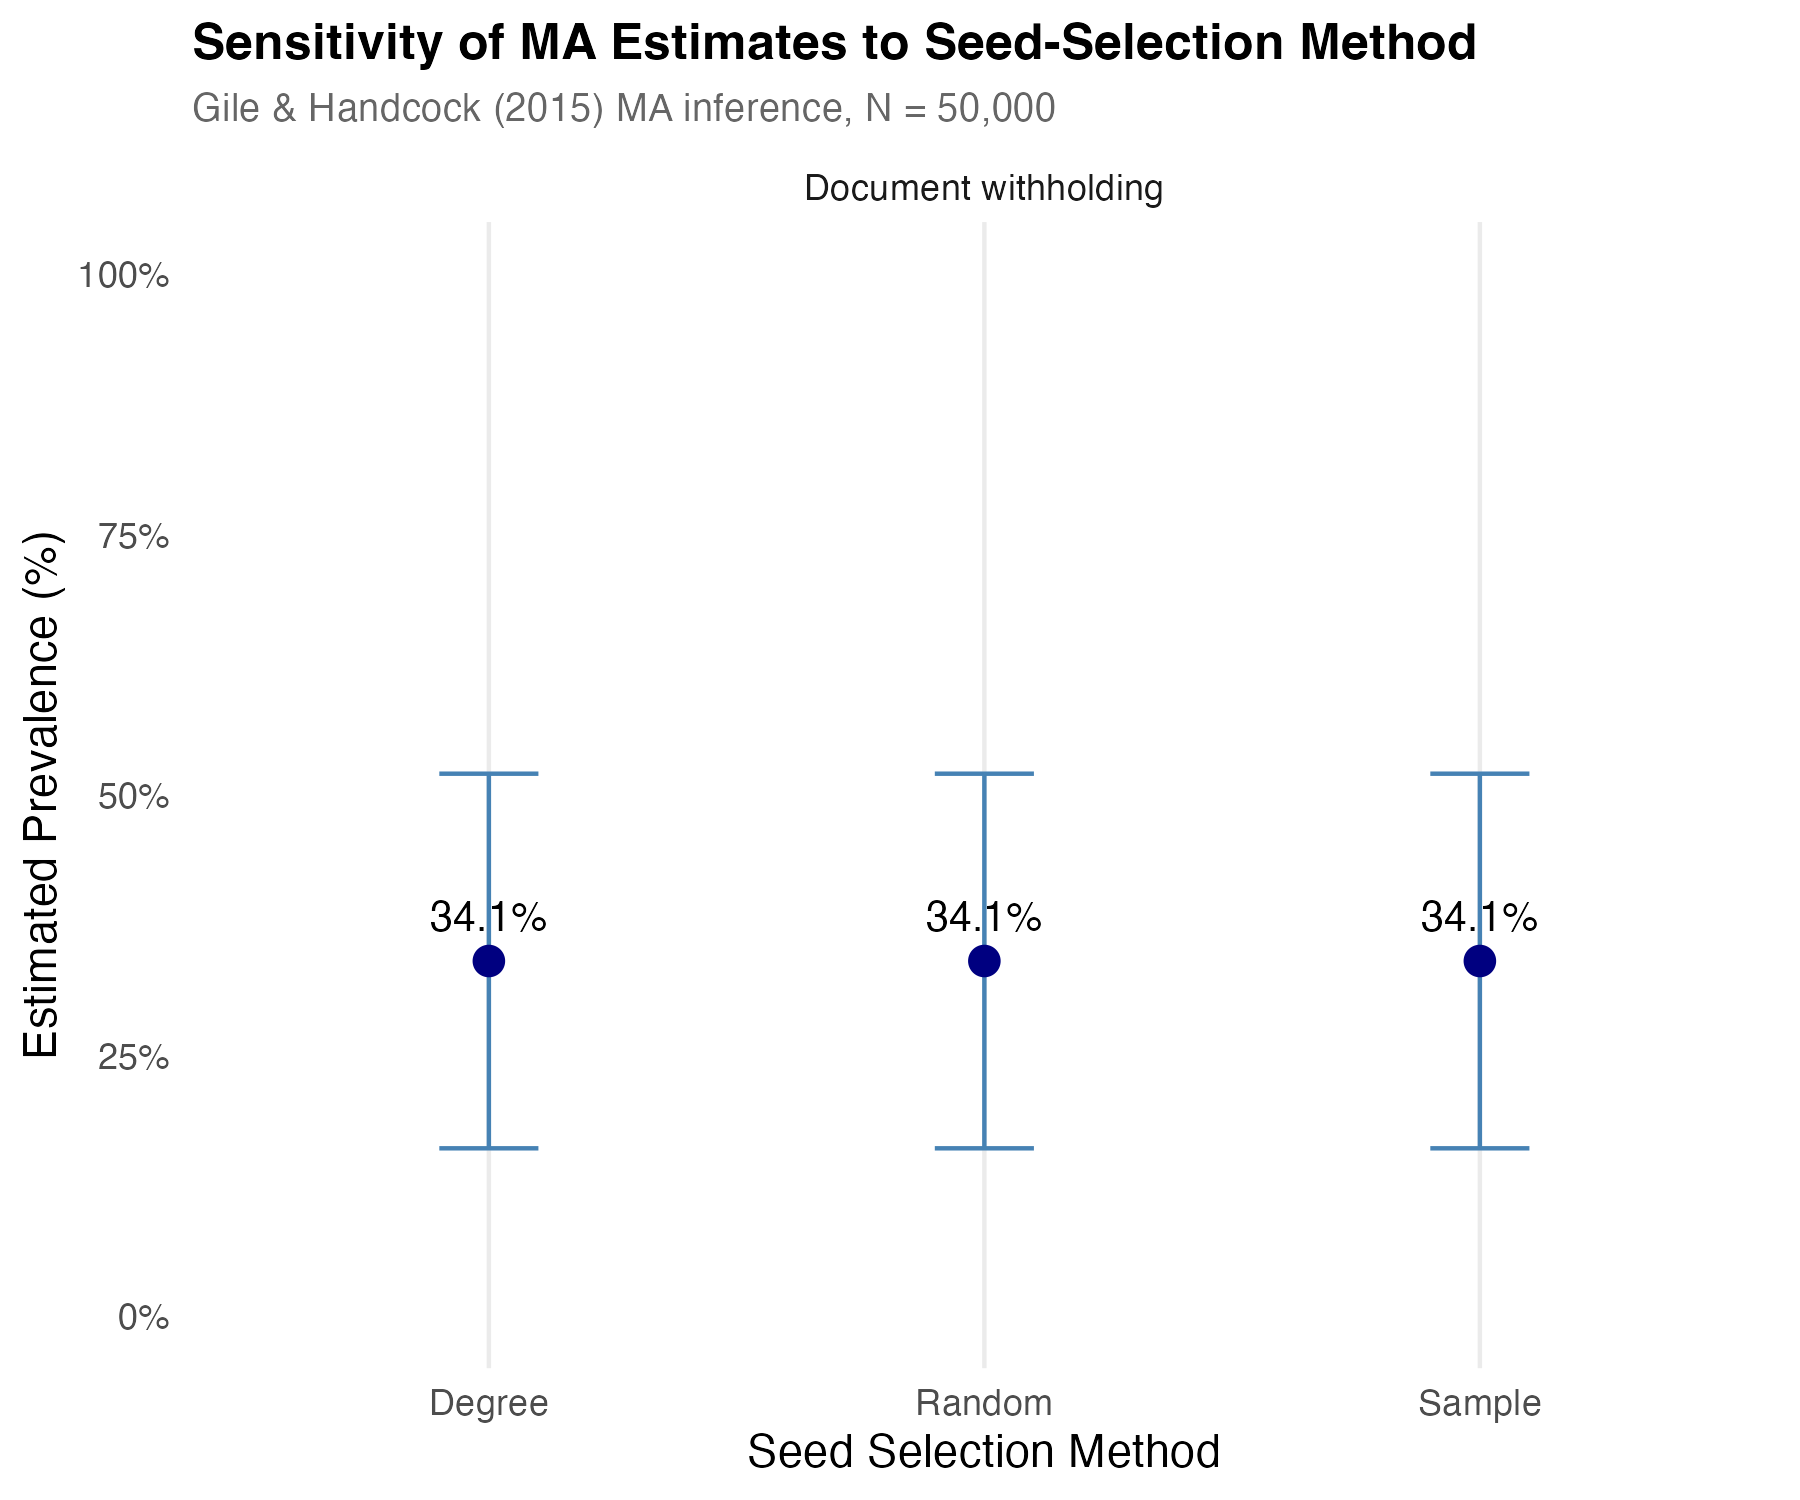
\includegraphics[width=5.5in,height=\textheight,keepaspectratio]{../figures/figA4_ma_seedcheck.png}

}

\caption{\label{fig-ma-seedcheck}Model-Assisted Seed-Selection
Sensitivity. Bayesian MA posterior estimates and 95\% credible intervals
for document withholding under three seed-selection methods (degree,
random, sample) at N = 50,000. All three methods converge to the same
posterior, supporting model robustness to initialisation. Source:
Authors' own work.}

\end{figure}%

\section{Supporting Estimates: RDS-I and RDS-SS
Comparison}\label{sec-d-rds-comp}

Table~\ref{tbl-rds-comparison} reports prevalence estimates and
neighbourhood-bootstrap 95\% confidence intervals for both the RDS-I
(Salganik--Heckathorn) and RDS-SS (Gile's Successive Sampling)
estimators across all four assumed population sizes. RDS-I runs
systematically higher than RDS-SS by 5--15 percentage points, consistent
with the standard finding that RDS-I is sensitive to seed dependence and
performs poorly at small sample sizes and shallow chain depths. The gap
between RDS-I and RDS-SS is larger for indicators where seed-cluster
homophily is strongest. Estimates are essentially invariant across
population sizes (confirming Section~\ref{sec-d-popsize}). The preferred
estimator for binary outcomes is RDS-SS; see main text Section 3.2.
Figure~\ref{fig-rds-comparison} visualises the RDS-I / RDS-SS gap across
the five indicators as paired point estimates with bootstrap CIs at
\(N = 980{,}000\), showing that RDS-I sits above RDS-SS for every
indicator with the largest gap for document withholding and the smallest
for limited access to help.

\begin{figure}[H]

\centering{

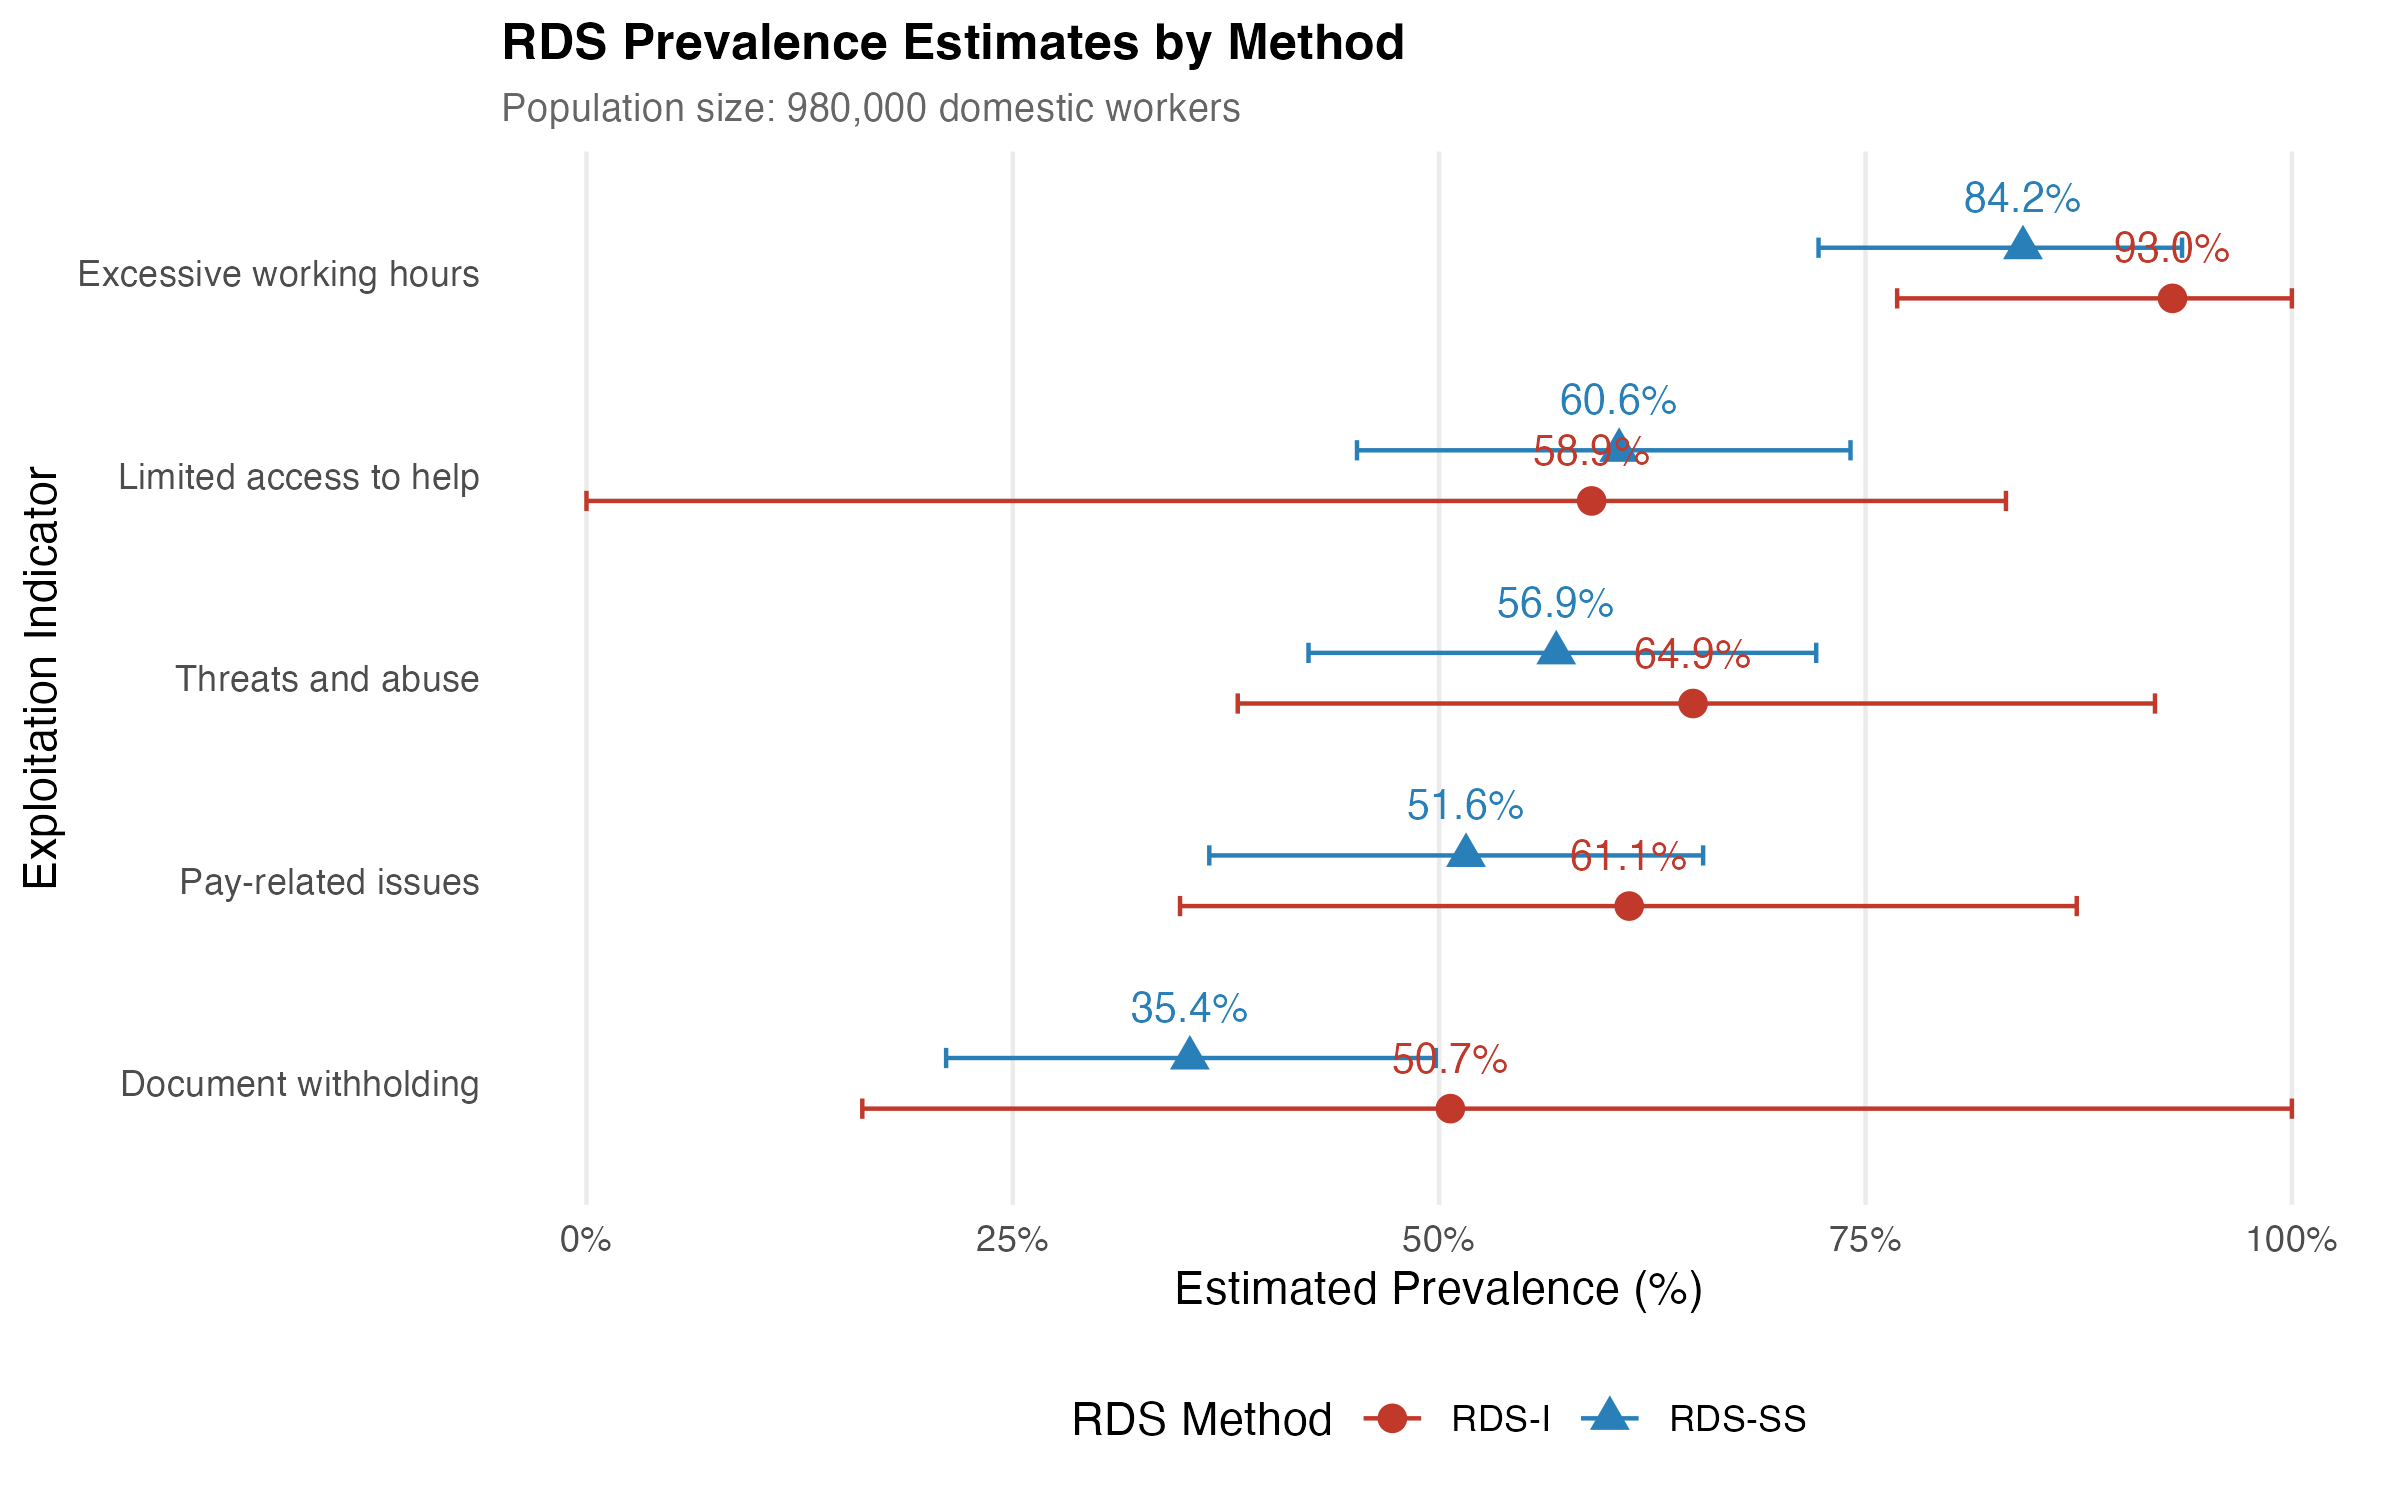
\includegraphics[width=6in,height=\textheight,keepaspectratio]{../figures/figA2_rds_comparison.png}

}

\caption{\label{fig-rds-comparison}RDS Prevalence Estimates by Method.
Neighbourhood-bootstrap 95\% confidence intervals for RDS-I
(Salganik--Heckathorn) and RDS-SS (Gile's Successive Sampling)
estimators for the five binary exploitation indicators, N = 980,000.
RDS-I runs systematically higher than RDS-SS by 5--15 percentage points,
consistent with seed dependence in the shallow-chain design. Source:
Authors' own work.}

\end{figure}%

\begin{longtable}[]{@{}
  >{\raggedright\arraybackslash}p{(\linewidth - 10\tabcolsep) * \real{0.1667}}
  >{\raggedright\arraybackslash}p{(\linewidth - 10\tabcolsep) * \real{0.1667}}
  >{\raggedright\arraybackslash}p{(\linewidth - 10\tabcolsep) * \real{0.1667}}
  >{\raggedright\arraybackslash}p{(\linewidth - 10\tabcolsep) * \real{0.1667}}
  >{\raggedright\arraybackslash}p{(\linewidth - 10\tabcolsep) * \real{0.1667}}
  >{\raggedright\arraybackslash}p{(\linewidth - 10\tabcolsep) * \real{0.1667}}@{}}
\caption{Comprehensive RDS Estimates: Both Estimators across All
Population Sizes. Neighbourhood-bootstrap 95\% CI in parentheses.
Estimates are invariant across N values; full table shows all four
population sizes for
completeness.}\label{tbl-rds-comparison}\tabularnewline
\toprule\noalign{}
\begin{minipage}[b]{\linewidth}\raggedright
Indicator
\end{minipage} & \begin{minipage}[b]{\linewidth}\raggedright
Estimator
\end{minipage} & \begin{minipage}[b]{\linewidth}\raggedright
N = 50,000
\end{minipage} & \begin{minipage}[b]{\linewidth}\raggedright
N = 100,000
\end{minipage} & \begin{minipage}[b]{\linewidth}\raggedright
N = 980,000
\end{minipage} & \begin{minipage}[b]{\linewidth}\raggedright
N = 1,740,000
\end{minipage} \\
\midrule\noalign{}
\endfirsthead
\toprule\noalign{}
\begin{minipage}[b]{\linewidth}\raggedright
Indicator
\end{minipage} & \begin{minipage}[b]{\linewidth}\raggedright
Estimator
\end{minipage} & \begin{minipage}[b]{\linewidth}\raggedright
N = 50,000
\end{minipage} & \begin{minipage}[b]{\linewidth}\raggedright
N = 100,000
\end{minipage} & \begin{minipage}[b]{\linewidth}\raggedright
N = 980,000
\end{minipage} & \begin{minipage}[b]{\linewidth}\raggedright
N = 1,740,000
\end{minipage} \\
\midrule\noalign{}
\endhead
\bottomrule\noalign{}
\endlastfoot
Document withholding & RDS-I & 49.4\% (25.3--56.3\%) & 49.4\%
(25.3--56.3\%) & 49.4\% (25.3--56.3\%) & 49.4\% (25.3--56.3\%) \\
Document withholding & RDS-SS & 34.2\% (25.2--56.0\%) & 34.2\%
(25.2--56.0\%) & 34.2\% (25.2--56.0\%) & 34.2\% (25.2--56.0\%) \\
Pay issues & RDS-I & 59.3\% (34.2--63.5\%) & 59.3\% (34.2--63.5\%) &
59.3\% (34.2--63.5\%) & 59.3\% (34.2--63.5\%) \\
Pay issues & RDS-SS & 49.7\% (34.8--63.4\%) & 49.7\% (34.8--63.4\%) &
49.7\% (34.8--63.4\%) & 49.7\% (34.8--63.4\%) \\
Threats and abuse & RDS-I & 65.2\% (40.5--72.1\%) & 65.2\%
(40.5--72.1\%) & 65.2\% (40.5--72.1\%) & 65.2\% (40.5--72.1\%) \\
Threats and abuse & RDS-SS & 57.2\% (40.1--72.3\%) & 57.2\%
(40.1--72.3\%) & 57.2\% (40.1--72.3\%) & 57.2\% (40.1--72.3\%) \\
Limited access to help & RDS-I & 57.7\% (55.1--80.3\%) & 57.7\%
(55.1--80.3\%) & 57.7\% (55.1--80.3\%) & 57.7\% (55.1--80.3\%) \\
Limited access to help & RDS-SS & 59.4\% (54.7--80.2\%) & 59.4\%
(54.7--80.2\%) & 59.4\% (54.7--80.2\%) & 59.4\% (54.7--80.2\%) \\
Excessive working hours & RDS-I & 92.8\% (71.4--92.9\%) & 92.8\%
(71.4--92.9\%) & 92.8\% (71.4--92.9\%) & 92.8\% (71.4--92.9\%) \\
Excessive working hours & RDS-SS & 83.7\% (71.5--93.0\%) & 83.7\%
(71.5--93.0\%) & 83.7\% (71.5--93.0\%) & 83.7\% (71.5--93.0\%) \\
\end{longtable}

\section{Supporting Estimates: NSUM under Alternative Adjustment-Factor
Tiers}\label{sec-d-nsum-tiers}

For comparison with the discrete-tier NSUM literature,
Table~\ref{tbl-nsum-tiers} reports MBSU prevalence under three reference
scenarios: Unadjusted (\(\delta = 1.0\), \(\tau = 1.0\)), Moderate
(\(\delta = 0.9\), \(\tau = 0.85\)), and Conservative (\(\delta = 0.8\),
\(\tau = 0.70\)). These correspond to three points on the continuous
sensitivity curve reported in Section~\ref{sec-d-tau-sweep}. The GNSUM
Symmetric estimator produces results identical to MBSU No Adjustment.
All estimates use \(N_F = 980{,}000\) and neighbourhood-bootstrap 95\%
CIs (\(B = 500\)). Figure~\ref{fig-nsum-forest} displays the MBSU
Moderate estimates as a forest plot: the five indicators all cluster in
the 1--3\% range under the Moderate adjustment scenario, with excessive
hours and pay issues at the top of the range and document withholding at
the bottom.

\begin{figure}[H]

\centering{

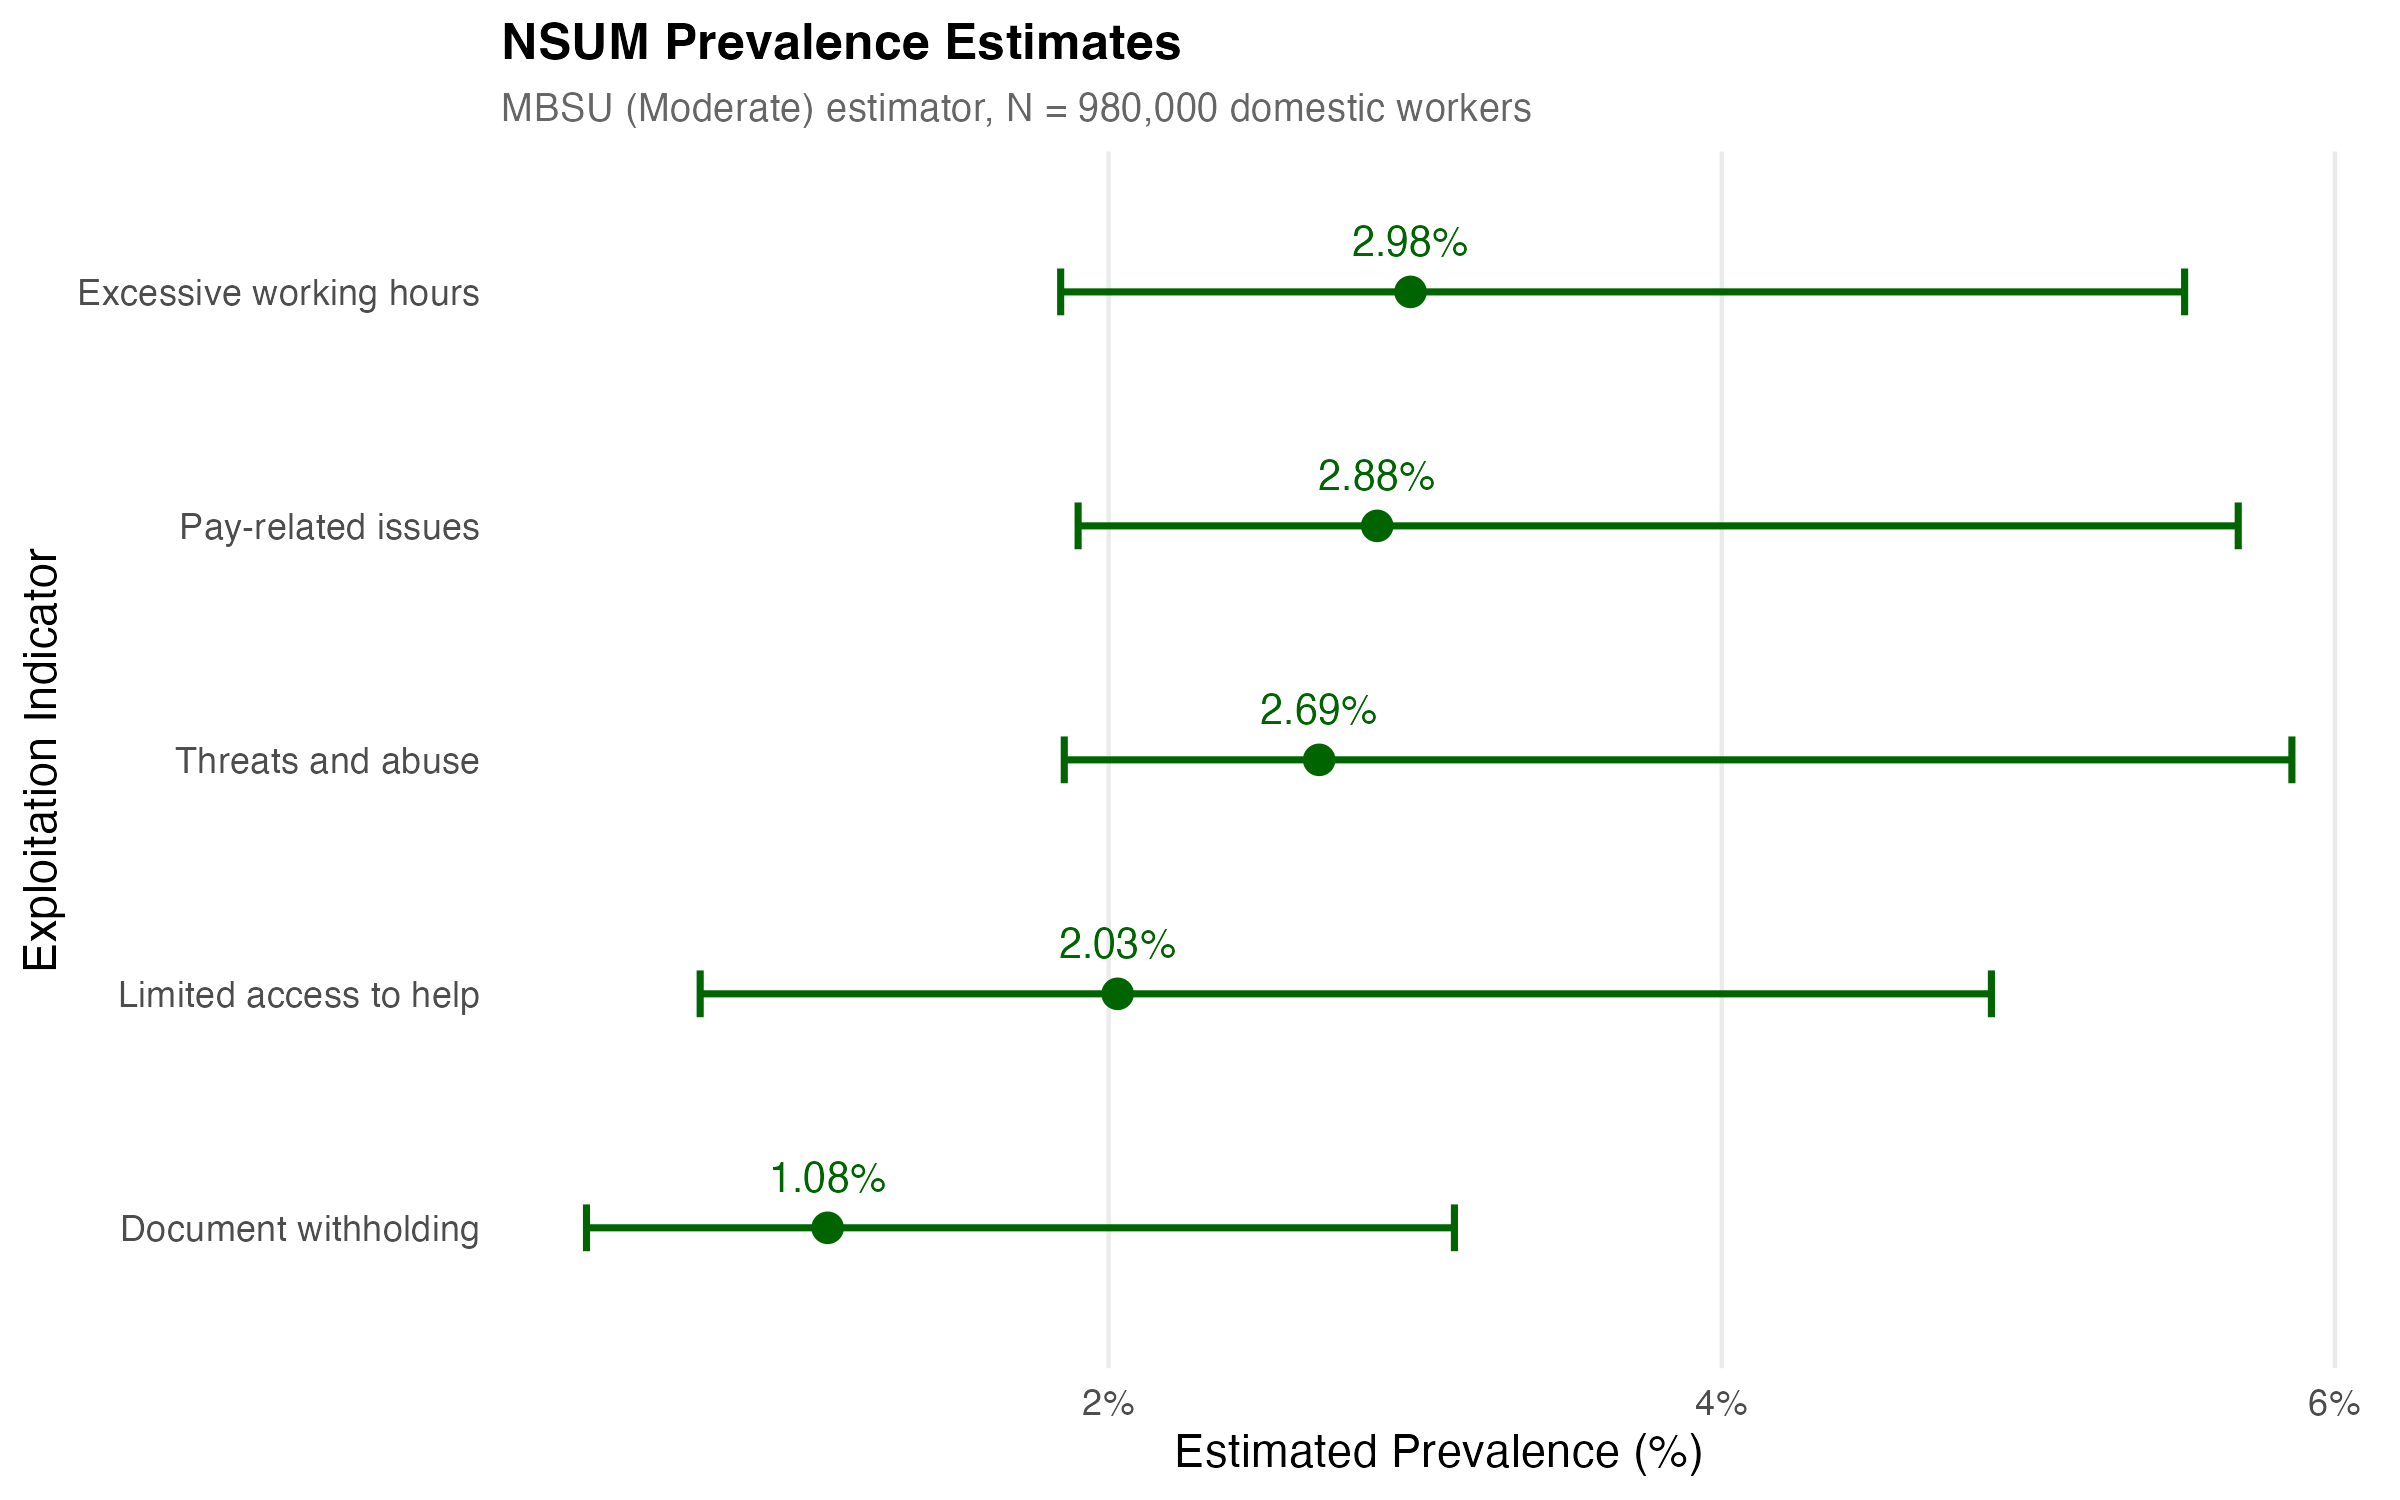
\includegraphics[width=5.5in,height=\textheight,keepaspectratio]{../figures/figA3_nsum_forest.png}

}

\caption{\label{fig-nsum-forest}NSUM (MBSU Moderate) Prevalence
Estimates. Forest plot of MBSU Moderate (\(\delta = 0.9\),
\(\tau = 0.85\)) prevalence estimates with neighbourhood-bootstrap 95\%
confidence intervals for the five binary exploitation indicators,
\(N_F = 980{,}000\). Source: Authors' own work.}

\end{figure}%

\begin{longtable}[]{@{}
  >{\raggedright\arraybackslash}p{(\linewidth - 4\tabcolsep) * \real{0.3333}}
  >{\raggedright\arraybackslash}p{(\linewidth - 4\tabcolsep) * \real{0.3333}}
  >{\raggedright\arraybackslash}p{(\linewidth - 4\tabcolsep) * \real{0.3333}}@{}}
\caption{NSUM Prevalence under Alternative Estimators and
Adjustment-Factor Scenarios, N = 980,000. Neighbourhood-bootstrap 95\%
CI in parentheses (B = 500). GNSUM Symmetric produces results identical
to MBSU No Adjustment.}\label{tbl-nsum-tiers}\tabularnewline
\toprule\noalign{}
\begin{minipage}[b]{\linewidth}\raggedright
NSUM method
\end{minipage} & \begin{minipage}[b]{\linewidth}\raggedright
Indicator
\end{minipage} & \begin{minipage}[b]{\linewidth}\raggedright
Prevalence (95\% CI)
\end{minipage} \\
\midrule\noalign{}
\endfirsthead
\toprule\noalign{}
\begin{minipage}[b]{\linewidth}\raggedright
NSUM method
\end{minipage} & \begin{minipage}[b]{\linewidth}\raggedright
Indicator
\end{minipage} & \begin{minipage}[b]{\linewidth}\raggedright
Prevalence (95\% CI)
\end{minipage} \\
\midrule\noalign{}
\endhead
\bottomrule\noalign{}
\endlastfoot
MBSU No Adjustment (δ=1.0, \(\tau\)=1.0) & Access to help & 1.55\%
(0.51--3.73\%) \\
MBSU No Adjustment (δ=1.0, \(\tau\)=1.0) & Document withholding & 0.83\%
(0.23--2.39\%) \\
MBSU No Adjustment (δ=1.0, \(\tau\)=1.0) & Excessive hours & 2.28\%
(1.41--4.21\%) \\
MBSU No Adjustment (δ=1.0, \(\tau\)=1.0) & Pay issues & 2.20\%
(1.45--4.35\%) \\
MBSU No Adjustment (δ=1.0, \(\tau\)=1.0) & Threats and abuse & 2.06\%
(1.42--4.48\%) \\
MBSU Moderate (δ=0.9, \(\tau\)=0.85) & Access to help & 2.03\%
(0.67--4.88\%) \\
MBSU Moderate (δ=0.9, \(\tau\)=0.85) & Document withholding & 1.08\%
(0.30--3.13\%) \\
MBSU Moderate (δ=0.9, \(\tau\)=0.85) & Excessive hours & 2.98\%
(1.84--5.51\%) \\
MBSU Moderate (δ=0.9, \(\tau\)=0.85) & Pay issues & 2.88\%
(1.90--5.68\%) \\
MBSU Moderate (δ=0.9, \(\tau\)=0.85) & Threats and abuse & 2.69\%
(1.86--5.86\%) \\
MBSU Conservative (δ=0.8, \(\tau\)=0.70) & Access to help & 2.77\%
(0.91--6.67\%) \\
MBSU Conservative (δ=0.8, \(\tau\)=0.70) & Document withholding & 1.48\%
(0.40--4.27\%) \\
MBSU Conservative (δ=0.8, \(\tau\)=0.70) & Excessive hours & 4.08\%
(2.52--7.53\%) \\
MBSU Conservative (δ=0.8, \(\tau\)=0.70) & Pay issues & 3.93\%
(2.60--7.77\%) \\
MBSU Conservative (δ=0.8, \(\tau\)=0.70) & Threats and abuse & 3.67\%
(2.53--8.00\%) \\
GNSUM Symmetric & Access to help & 1.55\% (0.51--3.73\%) \\
GNSUM Symmetric & Document withholding & 0.83\% (0.23--2.39\%) \\
GNSUM Symmetric & Excessive hours & 2.28\% (1.41--4.21\%) \\
GNSUM Symmetric & Pay issues & 2.20\% (1.45--4.35\%) \\
GNSUM Symmetric & Threats and abuse & 2.06\% (1.42--4.48\%) \\
\end{longtable}

\section{\texorpdfstring{Continuous-\(\tau\) NSUM Sensitivity
Sweep}{Continuous-\textbackslash tau NSUM Sensitivity Sweep}}\label{sec-d-tau-sweep}

The headline NSUM result in this paper is not the discrete-tier
comparison of Section~\ref{sec-d-nsum-tiers} but rather the continuous
sensitivity sweep: for each of the five exploitation indicators, MBSU
prevalence is shown as a continuous function of the
visibility/true-positive-rate adjustment parameter
\(\tau \in [0.40, 1.00]\), in increments of 0.05 (13 values), with
\(\delta\) fixed at 0.9 and \(B = 500\) neighbourhood-bootstrap 95\%
confidence intervals at each \(\tau\) value.

The three discrete tiers reported in Section~\ref{sec-d-nsum-tiers}
correspond to three points on these continuous curves: Unadjusted at
\(\tau = 1.0\), Moderate at \(\tau = 0.85\), and Conservative at
\(\tau = 0.70\). Prevalence increases monotonically as \(\tau\)
decreases (lower \(\tau\) means lower assumed visibility, hence the
estimator must scale up the raw alter-report count). The increase is
modest across the plausible range \(\tau \in [0.7, 1.0]\) and becomes
substantial only at \(\tau \leq 0.5\), which corresponds to an
assumption that fewer than half of true exploitation cases are visible
to the respondent's network --- an extreme scenario. The continuous
picture in Figure~\ref{fig-tau-sweep} supersedes the discrete-tier
comparison for substantive inference about how visibility assumptions
affect estimates: it makes explicit that the paper's conclusions about
indicator ordering and the RDS--NSUM visibility gradient are robust
across all plausible \(\tau\) values.

\begin{figure}[H]

\centering{

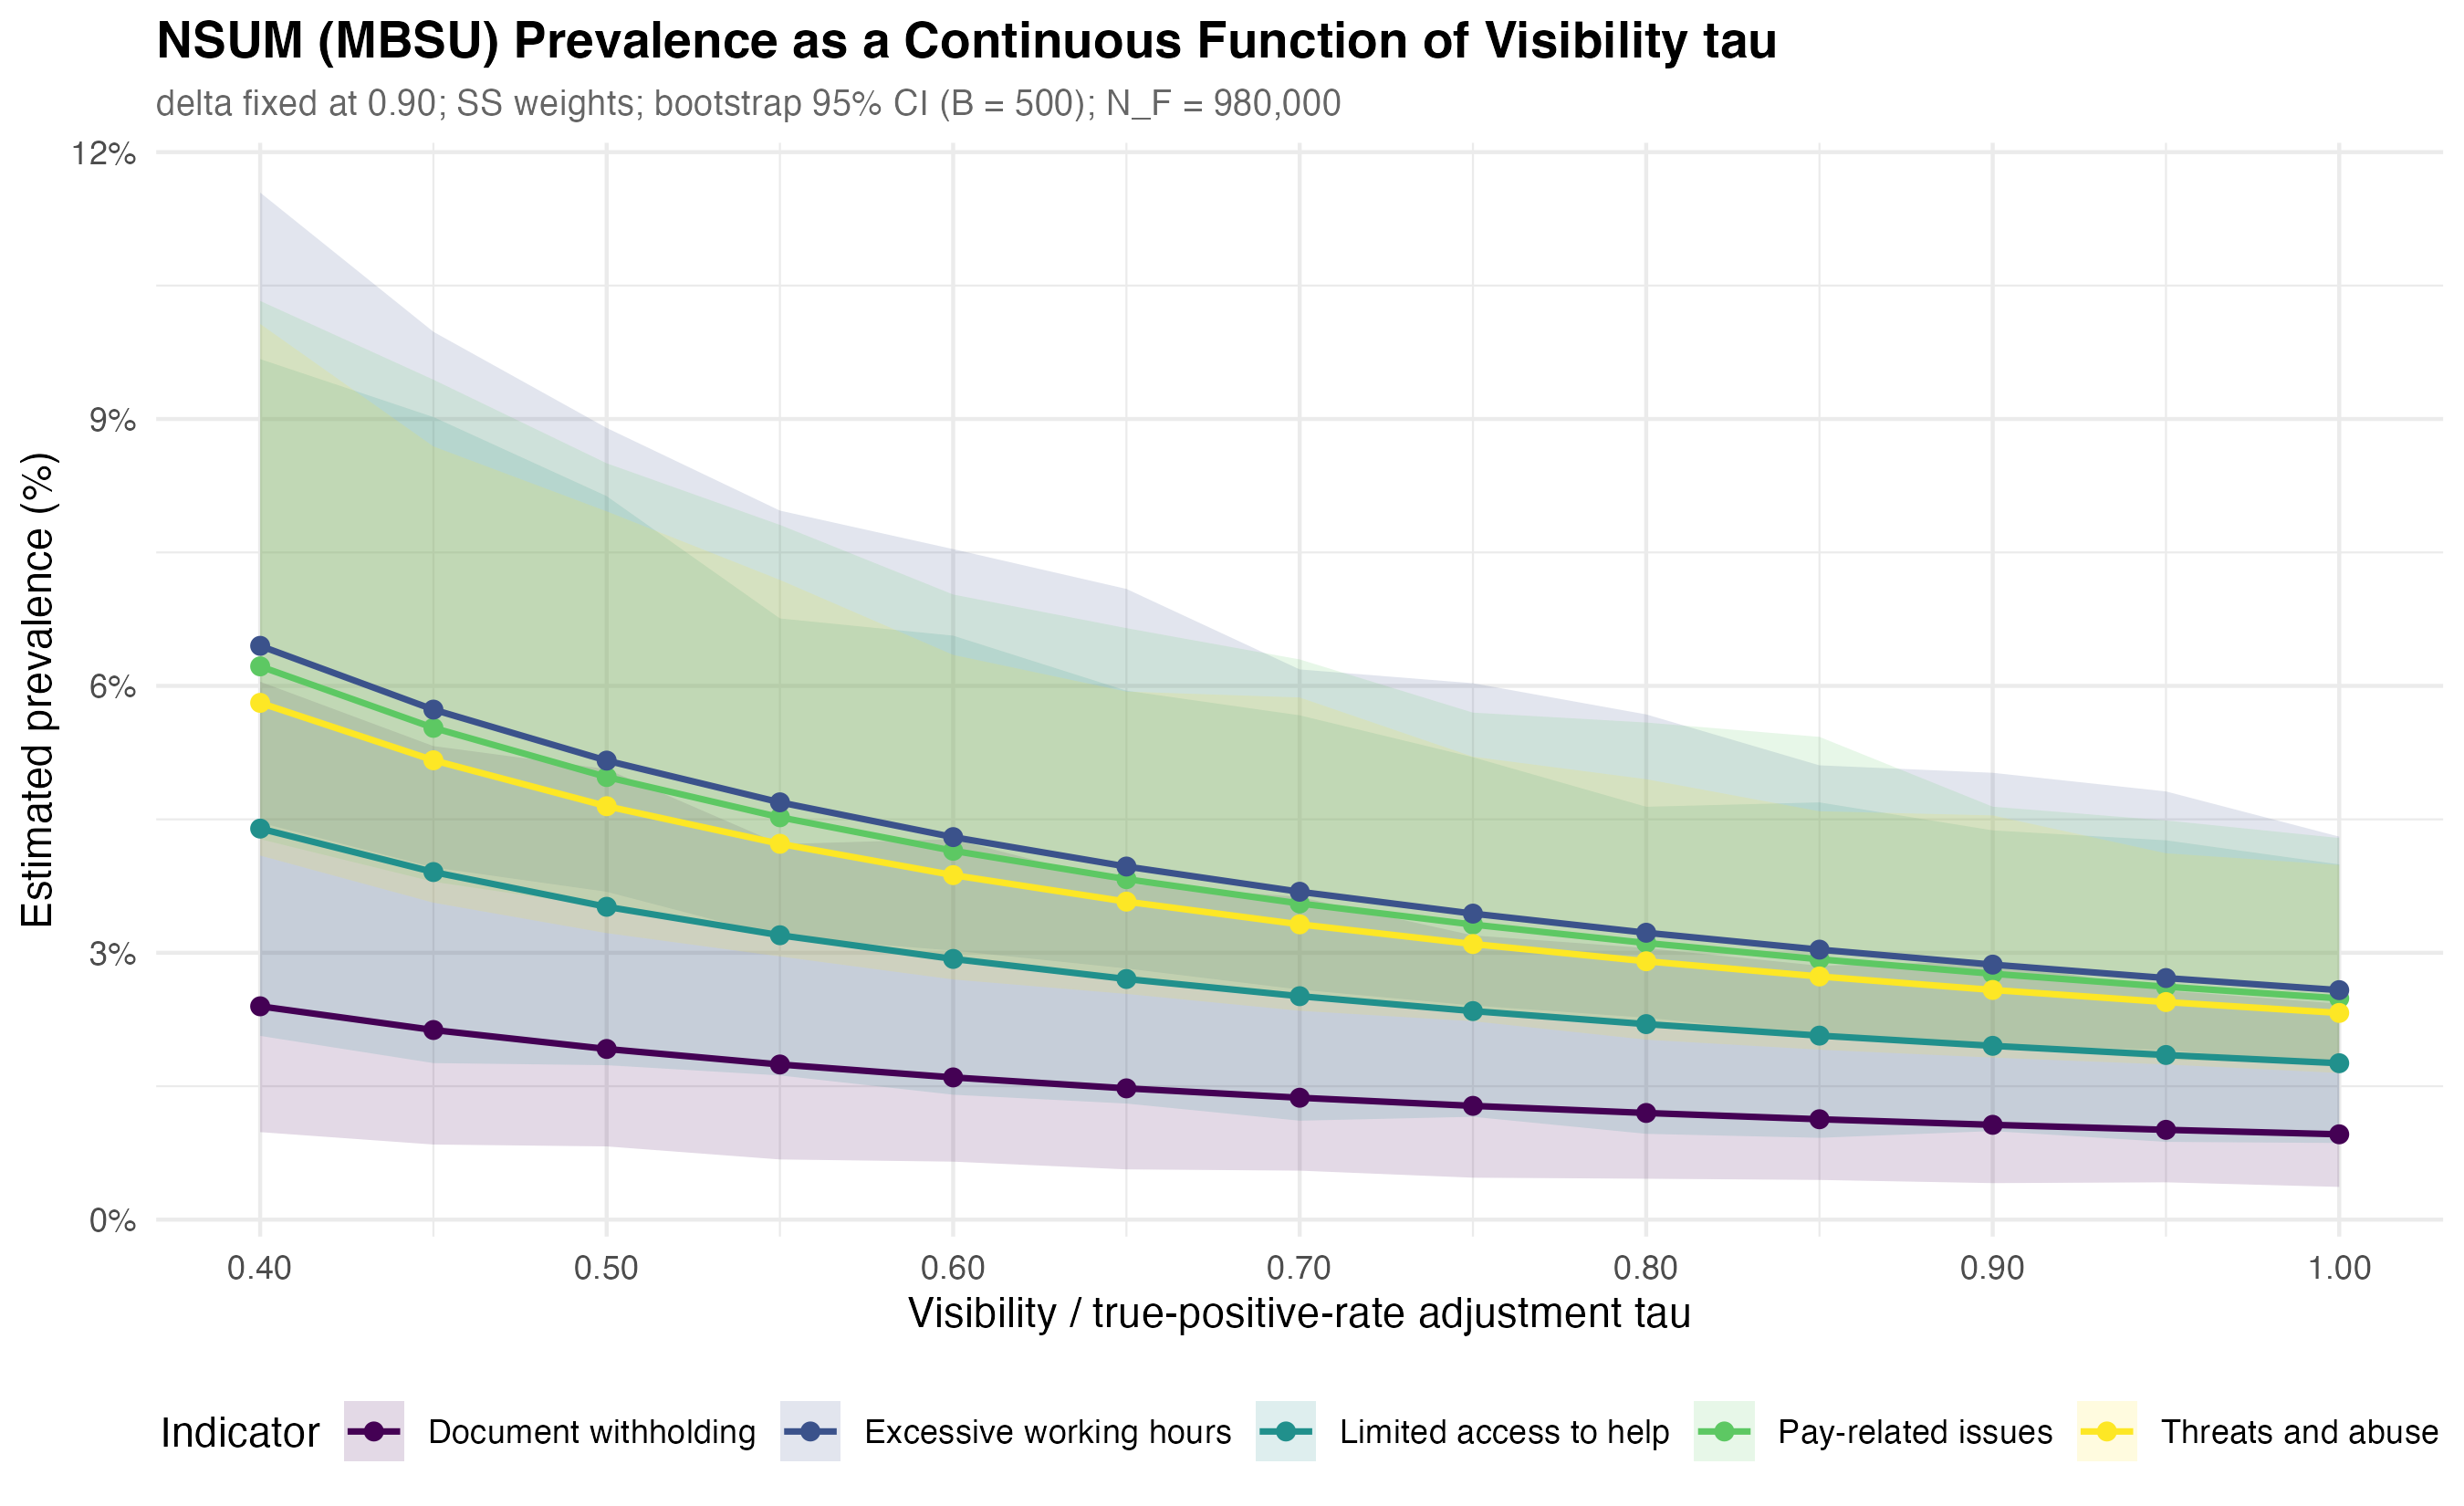
\includegraphics[width=6.5in,height=\textheight,keepaspectratio]{../figures/figA1_tau_sweep.png}

}

\caption{\label{fig-tau-sweep}NSUM (MBSU) Prevalence as a Continuous
Function of Visibility Parameter \(\tau\). MBSU prevalence estimates for
five exploitation indicators as a function of the
visibility/true-positive-rate adjustment \(\tau\), with δ fixed at 0.9
and B = 500 neighbourhood-bootstrap 95\% confidence intervals. Three
discrete scenarios from the main text (Unadjusted: \(\tau\) = 1.0;
Moderate: \(\tau\) = 0.85; Conservative: \(\tau\) = 0.70) correspond to
three points on each curve. N\_F = 980,000. Source: Authors' own work.}

\end{figure}%

\section{Robustness: Bootstrap Method and Weighting
Scheme}\label{sec-d-robustness}

Table~\ref{tbl-bootstrap-methods}, Table~\ref{tbl-weighting}, and
Table~\ref{tbl-popsize} confirm that the headline NSUM estimates are
robust to the choice of bootstrap resampling method, RDS weighting
scheme, and assumed population size. In all cases the MBSU Moderate
(\(\delta = 0.9\), \(\tau = 0.85\)) point estimates are identical across
variants; only confidence interval widths vary slightly across bootstrap
methods, and the differences are substantively negligible.

\begin{longtable}[]{@{}
  >{\raggedright\arraybackslash}p{(\linewidth - 4\tabcolsep) * \real{0.3333}}
  >{\raggedright\arraybackslash}p{(\linewidth - 4\tabcolsep) * \real{0.3333}}
  >{\raggedright\arraybackslash}p{(\linewidth - 4\tabcolsep) * \real{0.3333}}@{}}
\caption{Bootstrap Method Comparison. MBSU Moderate prevalence and
neighbourhood-bootstrap 95\% CI under four resampling methods. N =
980,000, SS weights. Point estimates identical across methods; CI widths
vary within ±0.5 percentage
points.}\label{tbl-bootstrap-methods}\tabularnewline
\toprule\noalign{}
\begin{minipage}[b]{\linewidth}\raggedright
Bootstrap method
\end{minipage} & \begin{minipage}[b]{\linewidth}\raggedright
Indicator
\end{minipage} & \begin{minipage}[b]{\linewidth}\raggedright
Prevalence (95\% CI)
\end{minipage} \\
\midrule\noalign{}
\endfirsthead
\toprule\noalign{}
\begin{minipage}[b]{\linewidth}\raggedright
Bootstrap method
\end{minipage} & \begin{minipage}[b]{\linewidth}\raggedright
Indicator
\end{minipage} & \begin{minipage}[b]{\linewidth}\raggedright
Prevalence (95\% CI)
\end{minipage} \\
\midrule\noalign{}
\endhead
\bottomrule\noalign{}
\endlastfoot
Chain & Access to help & 2.03\% (0.93--4.73\%) \\
Chain & Document withholding & 1.08\% (0.43--2.83\%) \\
Chain & Excessive hours & 2.98\% (2.07--5.39\%) \\
Chain & Pay issues & 2.88\% (1.99--5.08\%) \\
Chain & Threats and abuse & 2.69\% (1.92--4.85\%) \\
Neighbourhood (main analysis) & Access to help & 2.03\%
(0.67--4.88\%) \\
Neighbourhood (main analysis) & Document withholding & 1.08\%
(0.30--3.13\%) \\
Neighbourhood (main analysis) & Excessive hours & 2.98\%
(1.84--5.51\%) \\
Neighbourhood (main analysis) & Pay issues & 2.88\% (1.90--5.68\%) \\
Neighbourhood (main analysis) & Threats and abuse & 2.69\%
(1.86--5.86\%) \\
Successive Sampling & Access to help & 2.03\% (0.99--4.66\%) \\
Successive Sampling & Document withholding & 1.08\% (0.41--2.77\%) \\
Successive Sampling & Excessive hours & 2.98\% (2.13--5.27\%) \\
Successive Sampling & Pay issues & 2.88\% (2.06--4.94\%) \\
Successive Sampling & Threats and abuse & 2.69\% (1.92--4.56\%) \\
Tree & Access to help & 2.03\% (0.96--4.59\%) \\
Tree & Document withholding & 1.08\% (0.45--2.71\%) \\
Tree & Excessive hours & 2.98\% (2.09--5.40\%) \\
Tree & Pay issues & 2.88\% (2.06--5.05\%) \\
Tree & Threats and abuse & 2.69\% (1.91--4.70\%) \\
\end{longtable}

\begin{longtable}[]{@{}lll@{}}
\caption{Weighting Scheme Comparison. MBSU Moderate prevalence under
Successive Sampling (SS) and Volz--Heckathorn (VH) weights,
neighbourhood bootstrap, N = 980,000. SS and VH produce identical point
estimates and confidence intervals.}\label{tbl-weighting}\tabularnewline
\toprule\noalign{}
Weight scheme & Indicator & Prevalence (95\% CI) \\
\midrule\noalign{}
\endfirsthead
\toprule\noalign{}
Weight scheme & Indicator & Prevalence (95\% CI) \\
\midrule\noalign{}
\endhead
\bottomrule\noalign{}
\endlastfoot
SS (main analysis) & Access to help & 2.03\% (0.67--4.88\%) \\
SS (main analysis) & Document withholding & 1.08\% (0.30--3.13\%) \\
SS (main analysis) & Excessive hours & 2.98\% (1.84--5.51\%) \\
SS (main analysis) & Pay issues & 2.88\% (1.90--5.68\%) \\
SS (main analysis) & Threats and abuse & 2.69\% (1.86--5.86\%) \\
VH (Volz--Heckathorn) & Access to help & 2.03\% (0.67--4.88\%) \\
VH (Volz--Heckathorn) & Document withholding & 1.08\% (0.30--3.13\%) \\
VH (Volz--Heckathorn) & Excessive hours & 2.98\% (1.84--5.51\%) \\
VH (Volz--Heckathorn) & Pay issues & 2.88\% (1.90--5.68\%) \\
VH (Volz--Heckathorn) & Threats and abuse & 2.69\% (1.86--5.86\%) \\
\end{longtable}

\begin{longtable}[]{@{}lllll@{}}
\caption{Population Size Comparison. MBSU Moderate prevalence across
four assumed domestic-worker population sizes. Neighbourhood bootstrap,
SS weights. Prevalence is invariant across N values; absolute count
estimates scale proportionally with
N.}\label{tbl-popsize}\tabularnewline
\toprule\noalign{}
Indicator & N = 50,000 & N = 100,000 & N = 980,000 & N = 1,740,000 \\
\midrule\noalign{}
\endfirsthead
\toprule\noalign{}
Indicator & N = 50,000 & N = 100,000 & N = 980,000 & N = 1,740,000 \\
\midrule\noalign{}
\endhead
\bottomrule\noalign{}
\endlastfoot
Access to help & 2.03\% & 2.03\% & 2.03\% & 2.03\% \\
Document withholding & 1.08\% & 1.08\% & 1.08\% & 1.08\% \\
Excessive hours & 2.98\% & 2.98\% & 2.98\% & 2.98\% \\
Pay issues & 2.88\% & 2.88\% & 2.88\% & 2.88\% \\
Threats and abuse & 2.69\% & 2.69\% & 2.69\% & 2.69\% \\
\end{longtable}

\section{Survey Incentive Design}\label{sec-d-incentive}

The survey incentive structure followed the recommendations of Cobanoglu
\& Cobanoglu (\citeproc{ref-cobanoglu_effect_2003}{2003}), Brown et al.
(\citeproc{ref-brown_you_2006}{2006}), and Laguilles et al.
(\citeproc{ref-laguilles_can_2011}{2011}). A lottery entry into a free
prize draw for £150 was offered to all respondents completing the
questionnaire. Research by Gajic et al.
(\citeproc{ref-gajic_cost-effectiveness_2012}{2012}) suggests that a
high-value lottery provides the most cost-effective incentive for survey
participation in this type of study.

To minimise fraudulent responses, mobile phone numbers for each
respondent and those they referred were collated, and each was called by
one of the authors to verify respondent status as a domestic worker in
the UK. This verification step is particularly important in an RDS study
where respondents are recruited by peers, as it guards against chain
contamination.

The ethics of survey incentives for hidden and potentially vulnerable
populations have been carefully considered following Semaan et al.
(\citeproc{ref-semaan_ethical_2009}{2009}), DeJong et al.
(\citeproc{ref-dejong_ethical_2009}{2009}), and Singer \& Bossarte
(\citeproc{ref-singer_incentives_2006}{2006}). Our incentive design
follows the consensus recommendations of that literature: the incentive
is proportionate and not coercive; participation is voluntary; and
additional support resources were made available to respondents through
the partner organisations (Kalayaan and the Latin American Women's
Rights Service) who facilitated the data collection. Full ethical
approval was obtained prior to fieldwork.

\section{Leave-One-Out Chain Sensitivity}\label{sec-d-loo}

The main text notes that one chain (root seed \#55, length 12) accounts
for roughly a third of wave-2+ respondents, raising a question about
whether the rank ordering of exploitation indicators is driven by that
single chain. This section reports a leave-one-out (LOO) sensitivity
analysis in which the chain rooted at seed \#55 is entirely excluded,
and RDS-SS point estimates and 95\% bootstrap confidence intervals are
recomputed on the reduced sample.

\textbf{Chain identification.} Chain membership is determined by
breadth-first search (BFS) from the root node: starting with seed \#55,
all respondents whose \texttt{recruiter.id} traces back to seed \#55
(directly or transitively) are collected. The BFS is implemented in
\texttt{R/analysis/08c-loo\_chain\_analysis.R}. The chain contains 12
respondents --- seed \#55 plus 11 recruits spanning four subsequent
recruitment waves --- leaving a LOO analysis sample of \(n = 73\).
Table~\ref{tbl-loo-chain} lists the twelve excluded respondents; eleven
are Filipino and one is Latinx, and reported network degrees range from
0 to 30 (seed \#55 is the highest-degree node in the chain, though not
the highest-degree respondent in the whole sample).

\begin{longtable}[]{@{}
  >{\raggedright\arraybackslash}p{(\linewidth - 8\tabcolsep) * \real{0.2000}}
  >{\raggedright\arraybackslash}p{(\linewidth - 8\tabcolsep) * \real{0.2000}}
  >{\raggedright\arraybackslash}p{(\linewidth - 8\tabcolsep) * \real{0.2000}}
  >{\raggedright\arraybackslash}p{(\linewidth - 8\tabcolsep) * \real{0.2000}}
  >{\raggedright\arraybackslash}p{(\linewidth - 8\tabcolsep) * \real{0.2000}}@{}}
\caption{Excluded chain (seed \#55). Twelve respondents removed by the
LOO analysis, showing recruitment wave (0 = seed), self-reported network
degree (Q13), nationality cluster, and count of ILO-aligned binary
indicators reported affirmatively (of five). Ordered by wave then by
respondent id. Source: Authors' reconstruction from
\texttt{data/processed/prepared\_data.csv} via breadth-first search on
\texttt{recruiter.id}.}\label{tbl-loo-chain}\tabularnewline
\toprule\noalign{}
\begin{minipage}[b]{\linewidth}\raggedright
Respondent id
\end{minipage} & \begin{minipage}[b]{\linewidth}\raggedright
Wave
\end{minipage} & \begin{minipage}[b]{\linewidth}\raggedright
Degree (Q13)
\end{minipage} & \begin{minipage}[b]{\linewidth}\raggedright
Nationality
\end{minipage} & \begin{minipage}[b]{\linewidth}\raggedright
Indicators affirmed (of 5)
\end{minipage} \\
\midrule\noalign{}
\endfirsthead
\toprule\noalign{}
\begin{minipage}[b]{\linewidth}\raggedright
Respondent id
\end{minipage} & \begin{minipage}[b]{\linewidth}\raggedright
Wave
\end{minipage} & \begin{minipage}[b]{\linewidth}\raggedright
Degree (Q13)
\end{minipage} & \begin{minipage}[b]{\linewidth}\raggedright
Nationality
\end{minipage} & \begin{minipage}[b]{\linewidth}\raggedright
Indicators affirmed (of 5)
\end{minipage} \\
\midrule\noalign{}
\endhead
\bottomrule\noalign{}
\endlastfoot
55 (seed) & 0 & 30 & Filipino & 1 \\
41 & 1 & 5 & Filipino & 4 \\
63 & 1 & 5 & Filipino & 4 \\
6 & 2 & 10 & Filipino & 2 \\
10 & 2 & 2 & Filipino & 3 \\
42 & 2 & 10 & Filipino & 4 \\
44 & 2 & 5 & Filipino & 4 \\
12 & 3 & 0 & Filipino & 2 \\
18 & 3 & 10 & Latinx & 1 \\
90 & 3 & 1 & Filipino & 3 \\
45 & 4 & 10 & Filipino & 1 \\
64 & 4 & 10 & Filipino & 4 \\
\end{longtable}

\textbf{Re-estimation.} For each of the five comparable indicators,
RDS-SS estimates (Gile's Successive Sampling Horvitz-Thompson estimator)
are computed on (a) the full sample (\(n = 85\)) and (b) the LOO sample
(\(n = 73\)), using identical settings: \(N_F = 980{,}000\),
successive-sampling weights, neighbourhood-bootstrap 95\% CIs
(\(B = 500\)). The LOO \texttt{rds.data.frame} object is reconstructed
with the same parameters as the main analysis (network size variable:
\texttt{known\_network\_size}, max coupons: 5).

\textbf{Result.} Table~\ref{tbl-loo-comparison} reports the two sets of
estimates side by side; Figure~\ref{fig-loo} displays them as a paired
forest plot. Point-estimate shifts between the full and LOO samples
range from −3.2 to +4.5 percentage points across the five indicators,
and every LOO 95\% CI overlaps the corresponding full-sample CI. The top
and bottom of the ordering are preserved (document withholding lowest
and excessive hours highest in both samples), but the middle of the
ordering changes: \emph{threats and abuse} and \emph{limited access to
help} swap adjacent positions when seed \#55's chain is removed
(full-sample order: Doc \textless{} Pay \textless{} Threats \textless{}
Access \textless{} Excessive; LOO order: Doc \textless{} Pay \textless{}
Access \textless{} Threats \textless{} Excessive). Because the swap sits
entirely inside overlapping confidence intervals for both indicators, it
does not represent statistical evidence of a rank change; but it does
mean the ``rank order identical'' claim in earlier drafts of this
section overstates the robustness of the middle of the ordering. The LOO
sensitivity confirms the qualitative substantive claim --- that the
top-and-bottom prevalence structure is not driven by seed \#55's chain
--- while making explicit that adjacent-pair ordering in the middle of
the range depends on which chains happen to enter the sample.

\begin{longtable}[]{@{}
  >{\raggedright\arraybackslash}p{(\linewidth - 6\tabcolsep) * \real{0.2500}}
  >{\raggedright\arraybackslash}p{(\linewidth - 6\tabcolsep) * \real{0.2500}}
  >{\raggedright\arraybackslash}p{(\linewidth - 6\tabcolsep) * \real{0.2500}}
  >{\raggedright\arraybackslash}p{(\linewidth - 6\tabcolsep) * \real{0.2500}}@{}}
\caption{Full-sample vs Leave-One-Out RDS-SS Estimates. Preferred
prevalence estimates for the five binary ILO-aligned indicators on the
full sample (\(n = 85\)) and on the LOO sample with seed \#55's chain
excluded (\(n = 73\)). Neighbourhood-bootstrap 95\% confidence intervals
in parentheses. \(N_F = 980{,}000\), SS weights, \(B = 500\). All five
full-vs-LOO CI pairs overlap. Source:
\texttt{output/tables/loo\_chain\_sensitivity.csv}.}\label{tbl-loo-comparison}\tabularnewline
\toprule\noalign{}
\begin{minipage}[b]{\linewidth}\raggedright
Indicator
\end{minipage} & \begin{minipage}[b]{\linewidth}\raggedright
Full sample (n = 85)
\end{minipage} & \begin{minipage}[b]{\linewidth}\raggedright
LOO sample (n = 73)
\end{minipage} & \begin{minipage}[b]{\linewidth}\raggedright
Shift (pp)
\end{minipage} \\
\midrule\noalign{}
\endfirsthead
\toprule\noalign{}
\begin{minipage}[b]{\linewidth}\raggedright
Indicator
\end{minipage} & \begin{minipage}[b]{\linewidth}\raggedright
Full sample (n = 85)
\end{minipage} & \begin{minipage}[b]{\linewidth}\raggedright
LOO sample (n = 73)
\end{minipage} & \begin{minipage}[b]{\linewidth}\raggedright
Shift (pp)
\end{minipage} \\
\midrule\noalign{}
\endhead
\bottomrule\noalign{}
\endlastfoot
Document withholding & 35.4\% (20.3--48.1\%) & 33.4\% (17.5--48.8\%) &
−2.0 \\
Pay/debt issues & 51.6\% (37.2--65.9\%) & 55.3\% (41.0--71.0\%) &
+3.8 \\
Threats and abuse & 56.9\% (41.7--71.3\%) & 61.4\% (46.5--76.7\%) &
+4.5 \\
Excessive hours & 84.2\% (72.9--94.1\%) & 82.5\% (69.7--93.7\%) &
−1.7 \\
Limited access to help & 60.6\% (45.4--73.2\%) & 57.3\% (41.3--72.6\%) &
−3.2 \\
\end{longtable}

\begin{figure}[H]

\centering{


\includegraphics[width=6in,height=\textheight,keepaspectratio]{../figures/figA5_loo_chain.png}

}

\caption{\label{fig-loo}Leave-One-Out Chain Sensitivity. RDS-SS point
estimates and neighbourhood-bootstrap 95\% confidence intervals for the
five exploitation indicators in the full sample (n = 85) and in the LOO
sample with seed \#55's chain excluded (n = 73). N = 980,000. Source:
Authors' own work.}

\end{figure}%

\phantomsection\label{refs}
\begin{CSLReferences}{1}{0}
\bibitem[\citeproctext]{ref-brown_you_2006}
Brown, J. S., Schonfeld, T. L., \& Gordon, B. G. (2006). You may have
already won...'': An examination of the use of lottery payments in
research. \emph{{IRB}: Ethics \& Human Research}, \emph{28}(1), 12--16.

\bibitem[\citeproctext]{ref-cobanoglu_effect_2003}
Cobanoglu, C., \& Cobanoglu, N. (2003). The effect of incentives in web
surveys: Application and ethical considerations. \emph{International
Journal of Market Research}, \emph{45}(4), 1--13.
\url{https://doi.org/10.1177/147078530304500406}

\bibitem[\citeproctext]{ref-dejong_ethical_2009}
DeJong, J., Mahfoud, Z., Khoury, D., Barbir, F., \& Afifi, R. A. (2009).
Ethical considerations in {HIV}/{AIDS} biobehavioral surveys that use
respondent-driven sampling: Illustrations from lebanon. \emph{American
Journal of Public Health}, \emph{99}(9), 1562--1567.
\url{https://doi.org/10.2105/AJPH.2007.130773}

\bibitem[\citeproctext]{ref-feeh16-generalizing}
Feehan, D. M., \& Salganik, M. J. (2016). Generalizing the {Network
Scale-Up Method}: {A New Estimator} for the {Size} of {Hidden
Populations}. \emph{Sociological Methodology}, \emph{46}(1), 153--186.

\bibitem[\citeproctext]{ref-gajic_cost-effectiveness_2012}
Gajic, A., Cameron, D., \& Hurley, J. (2012). The cost-effectiveness of
cash versus lottery incentives for a web-based, stated-preference
community survey. \emph{The European Journal of Health Economics},
\emph{13}(6), 789--799. \url{https://doi.org/10.1007/s10198-011-0332-0}

\bibitem[\citeproctext]{ref-gile_network_2015}
Gile, K. J., \& Handcock, M. S. (2015). Network model-assisted inference
from respondent-driven sampling data. \emph{Journal of the Royal
Statistical Society: Series A (Statistics in Society)}, \emph{178}(3),
619--639. \url{https://doi.org/10.1111/rssa.12091}

\bibitem[\citeproctext]{ref-ILO11-indicators}
International Labour Organization. (2012). \emph{ILO indicators of
forced labour}. International Labour Organization.
\url{https://www.ilo.org/publications/ilo-indicators-forced-labour}

\bibitem[\citeproctext]{ref-hard24-ilo}
International Labour Organization. (2024). \emph{Hard to see, harder to
count handbook on forced labour surveys} (Third Edition). International
Labour Organization. \url{https://www.ilo.org/forcedlabour}

\bibitem[\citeproctext]{ref-int25-ilo}
International Labour Organization. (2025). \emph{ILO indicators of
forced labour} {[}2025 revised edition{]}. International Labour
Organization. \url{https://www.ilo.org/forcedlabour}

\bibitem[\citeproctext]{ref-laguilles_can_2011}
Laguilles, J. S., Williams, E. A., \& Saunders, D. B. (2011). Can
lottery incentives boost web survey response rates? Findings from four
experiments. \emph{Research in Higher Education}, \emph{52}(5),
537--553. \url{https://doi.org/10.1007/s11162-010-9203-2}

\bibitem[\citeproctext]{ref-semaan_ethical_2009}
Semaan, S., Santibanez, S., Garfein, R. S., Heckathorn, D. D., \&
Jarlais, D. C. (2009). Ethical and regulatory considerations in {HIV}
prevention studies employing respondent-driven sampling.
\emph{International Journal of Drug Policy}, \emph{20}(1), 14--27.
\url{https://doi.org/10.1016/j.drugpo.2007.12.006}

\bibitem[\citeproctext]{ref-singer_incentives_2006}
Singer, E., \& Bossarte, R. M. (2006). Incentives for survey
participation: When are they {``coercive''}? \emph{American Journal of
Preventive Medicine}, \emph{31}(5), 411--418.
\url{https://doi.org/10.1016/j.amepre.2006.07.013}

\bibitem[\citeproctext]{ref-yauck_neighboot_2022}
Yauck, M., \& Moodie, E. E. M. (2022). \emph{Neighboot: Neighborhood
bootstrap method for {RDS}} (Version 1.0.1) {[}Computer software{]}.
\url{https://cran.r-project.org/web/packages/Neighboot/index.html}

\end{CSLReferences}




\end{document}
